\section{Многоквантовая спектроскопия ЯМР}
% JMR-2020
Среди различных модельных физических систем,
рассматриваемых для реализации устройств и систем квантовой обработки информации,
ядерные спины обладают исключительной изоляцией от внешней среды
и широкими возможностями для манипулирования радиочастотными импульсами.
Многоквантовая (MK) спектроскопия ЯМР~\cite{Baum1985} позволяет создавать многоквантовые состояния,
а также экспериментально отслеживать процесс их релаксации.
%Одним из таких экспериментов является многоквантовый (МК) ЯМР в системах спинов,
%связанных прямым диполь-дипольным взаимодействием (DDI).
Приложения МК спектроскопии ЯМР включают широкий спектр неорганических и органических твердых тел и жидких кристаллов~\cite{Hughes2004}.
МК спектроскопия ЯМР может использоваться для решения вопроса о распределении атомов в материалах
и особенно хорошо подходит для анализа сложных по составу и неупорядоченных систем~\cite{Vasilev2018, Avilova2019, Mogami2014}.
МК ЯМР может быть использован для изучения декогеренции в системах,
состоящих из большого числа коррелированных спинов~\cite{Krojanski2006, Cho2006},
что открывает возможности для установления связи между числом частиц и скоростью декогеренции~\cite{Krojanski2006, Bochkin2018}.
Метод позволяет следить за распространением корреляций~\cite{Baum1985, Sanchez2014}
и наблюдать явления локализации в системах многих тел~\cite{Alvarez2015, Wei2018}.
Скорость распространения может быть описана через неупорядоченные по времени корреляторы
(``out-of-time-ordered correlators''~OTOCs),
которые связаны с распределением интенсивности когерентностей МК ЯМР~\cite{Garttner2018, Doronin2019}.

% Многоквантовая спектроскопия ЯМР служит эффективным методом для изучения распределения ядерных спинов в жидких кристаллах [2],
% в простых органических соединениях [1],
% в аморфном гидрированном кремнии [3] и т.д.
% Многоквантовый ЯМР успешно применяется [4, 5] для исследования размеров спиновых кластеров
% при их росте в процессе облучения спиновой системы радиочастотными (РЧ) импульсами на подготовительном периоде многоквантового эксперимента ЯМР [1].
% Недавно уникальные возможности многоквантового ЯМР были использованы [6, 7] для определения зависимости скорости декогеренции сильно коррелированных спиновых состояний от числа коррелированных спинов.

Многоквантовая динамика ядерного магнитного резонанса (ЯМР) является основой многоквантовой спектроскопии ЯМР~\cite{Baum1985}.
В обычных экспериментах ЯМР происходят лишь переходы между зеемановскими уровнями
с изменением проекции спинового момента на направление внешнего магнитного поля на $\pm 1$.
В результате основные наблюдаемые (например, спад свободной индукции) определяются относительно небольшим количеством отличных от нуля элементов матрицы плотности.
В многоквантовых экспериментах ЯМР,
где, в принципе, возможны переходы между любыми уровнями,
состояние спиновой системы определяется всеми элементами матрицы плотности.
Таким образом, информационный ресурс многоквантового ЯМР превосходит ресурс обычного ЯМР.

Теоретическое описание многоквантовой динамики ЯМР является сложной задачей, которая сводится к анализу многочастичную и многоквантовой системы. Матрицу плотности системы в многоквантовом эксперименте ЯМР можно представлять суммой членов, каждый из которых содержит тензорные произведения односпиновых операторов
(например, для $k$~-спина это $I_{kz}$,
$I_k^+ = I_{kx} + iI_{ky}$, $I_k^+ = I_{kx} - iI_{ky}$,
ось квантования $z$ --- направление внешнего магнитного поля,
$I_{k\alpha}$ --- проекция углового спинового момента на ось $\alpha$,
$\alpha=x,y,z$.
Разность числа повышающих и понижающих операторов, содержащихся в члене, определяет порядок многоквантовой когерентности, за которую этот член отвечает.
В многоквантовой спектроскопии ЯМР~\cite{Baum1985} наблюдаются интенсивности различных многоквантовых когерентностей.
Задача теории состоит в их вычислении.

В многоквантовом эксперименте ЯМР спиновая
система облучается периодической последовательностью резонансных радиочастотных импульсов.
Если обратный период облучающей последовательности $t_{c}^{-1}$
значительно превосходит величину усредняемых взаимодействий
$\omega_\mathrm{loc} (\epsilon = t_{c}\, \omega_\mathrm{loc} \ll 1)$,
то анизотропные диполь-дипольные взаимодействия~\cite{Goldman1970} становятся быстроосциллирующими.
Теория среднего гамильтониана ~\cite{Haberlen1969} позволяет найти усредненные взаимодействия,
гамильтониан которых $H_{MQ}$ (несекулярный двухспиновый/двухквантовый гамильтониан~\cite{Baum1985})
с точностью до членов порядка $\epsilon^2$ имеет вид:
\begin{equation}\label{eq:hmq}
    H_{MQ} = H^{(2)} + H^{(-2)},
    \quad
    H^{(\pm2)} = \frac 1 2 \sum_{i < j} D_{ij} I^\pm_i I^\pm_j,
\end{equation}
где $D_{ij}$ --- константа диполь-дипольного взаимодействия спинов $i$ и $j$, а $I^\pm_i = I_{ix} \pm iI_{iy}$.


\subsection{Многоквантовый эксперимент ЯМР}\label{sec:mq-nrm-experiment}
% Многоквантовый эксперимент ЯМ~\cite{Baum1985}
%

%
% На подготовительном периоде МК эксперимента ЯМР система облучается последовательностью радиочастотных импульсов. В результате динамика спиновой системы определяется многоквантовым гамильтонианом.
%
% $$
% H_{MQ} = H^{(2)} + H^{(-2)},
% \quad H^{(\pm2)} = \frac 1 2 \sum_{i < j} D_{ij} I^\pm_i I^\pm_j
% $$
%
%  МК динамику мы решили исследовать стандартным МК экспериментом.
%  Эксперимент состоит из четырех частей,
%  но нас будет интересовать только подготовительный период эксперимента.
%  На подготовительном периоде ...слайд...
%
% Многоквантовый экперимент ЯМР
%

%
%     МК когерентности создаются в течение периода подготовки продолжительностью $\tau$ при участии m-серии 8-импульсовых подпоследовательностей и затем преобразуются в наблюдаемую намагниченность после идентичного периода смешивания (за исключением 90-градусного фазового сдвига). Затем намагниченность детектируется при импульсе $\pi/2$. Фазовый сдвиг $\phi$ между периодами подготовки и смешивания инкриминируется для разделения многоквантовых когерентностей разных порядков. В результате преобразования Фурье по $\phi$ получается МК ЯМР спектр. Интенсивности МК когерентностей ЯМР при различных длительностях периода свободной эволюции $t$ получаются в отдельных экспериментах.
%
%
% \begin{figure}
%   \centering
%   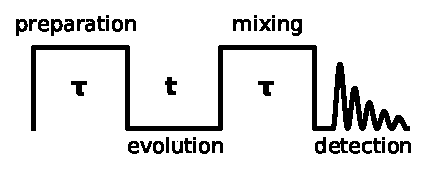
\includegraphics[width=0.5\textwidth]{mq-experiment-schema.pdf}
%   \caption{Схема МК эксперимента ЯМР}
% \end{figure}
\begin{figure}
  \centering
  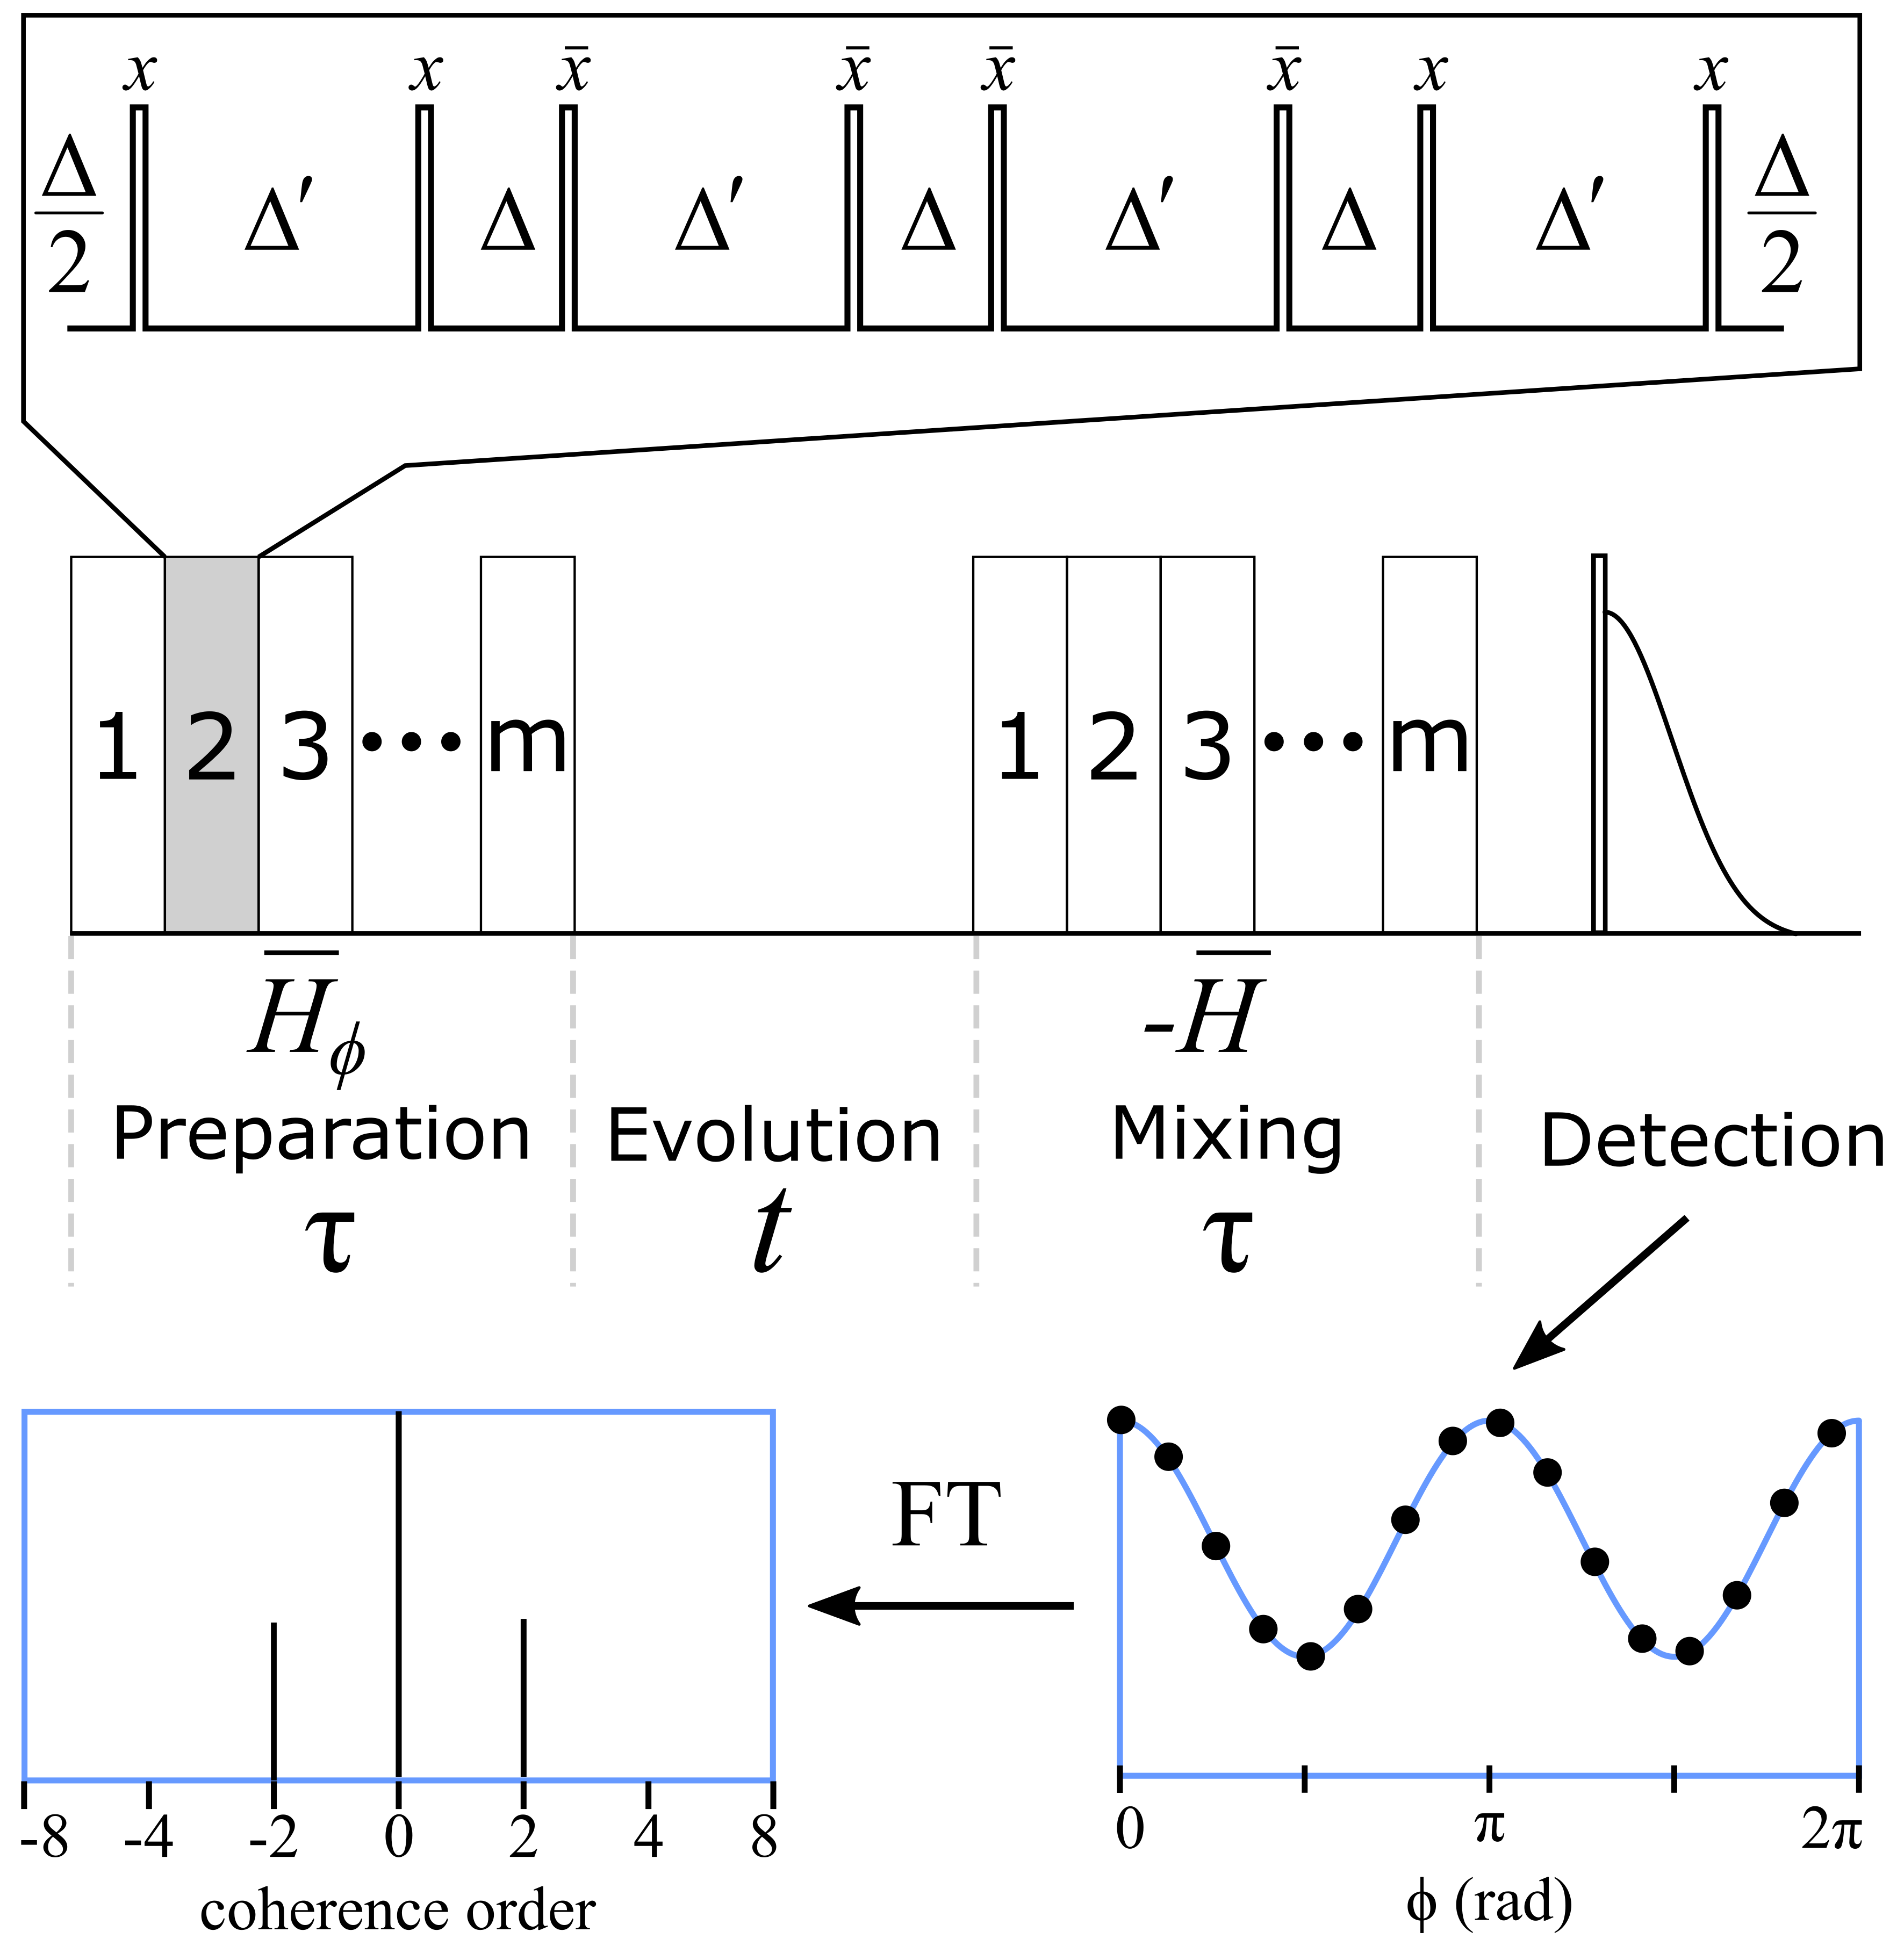
\includegraphics[width=0.5\textwidth]{mq-experiment-pulses-schema.png}
  \caption{Схема МК эксперимента ЯМР}
  \label{fig:mq-experiment-pulses-schema}
\end{figure}

Многоквантовый эксперимент ЯМР состоит из четырех основных периодов (Рис.~\ref{fig:mq-experiment-pulses-schema}): подготовительного, свободной эволюции, смешивания и детектирования.
Эти периоды многократно повторяются с инкрементом фазы РЧ-импульсов, облучающих спиновую систему на подготовительном периоде при каждом повторении. Используемая последовательность РЧ-импульсов построена из базовых циклов, состоящих из восьми резонансных $\pi/2$-импульсов (Рис.~\ref{fig:mq-experiment-pulses-schema}).
На подготовительном периоде многоквантового эксперимента ЯМР
система облучается несколькими такими циклами,
что приводит к возникновению многоквантовых когерентностей четного порядка.
При инкременте фазы РЧ-импульсов $\varphi$ несекулярный двухспиновый/двухквантовый гамильтониан~(\ref{eq:hmq}) принимает следующий вид:
%
\begin{equation}\label{eq:hmq-phased}
    H_\mathrm{MQ}^{\phi} = e^{-2i\phi}H^{(2)} + e^{2i\phi}H^{(-2)}.
\end{equation}
%
Использование инкремента фазы РЧ-импульсов позволяет разделить сигналы от многоквантовых когерентностей разных порядков на периоде свободной эволюции~\cite{Shykind1988} (Рис.~\ref{fig:mq-experiment-pulses-schema}).

Поскольку многоквантовые когерентности ЯМР не могут наблюдаться непосредственно, они преобразуются в поперечную намагниченность (одноквантовую когерентность) на периоде смешивания. На периоде смешивания спиновая система облучается такой же последовательностью РЧ-импульсов, как и на подготовительном периоде, но фаза импульсов сдвигается на $\pi/2$
(вместо $x$-импульсов подаются  $y$-импульсы).
Формула~(\ref{eq:hmq-phased}) показывает, что при таком сдвиге фазы изменяется знак несекулярного двухспинового/двухквантового гамильтониана~(\ref{eq:hmq}).
Таким образом, на периоде смешивания создаются условия обращения времени~\cite{Rhim1971},
необходимые для сфазирования вкладов разных пар спинов в многоквантовые когерентности разных порядков~\cite{Baum1985}.
%
Матрица плотности системы после периода смешивания может быть записана как~\cite{Baum1985}
\begin{equation}\label{eq:rho-after-mixing}
  \rho_\mathrm{f}(\tau)
  = e^{i{H_{MQ}}\tau} e^{i\phi I_z} e^{-i{ H_{MQ}}\tau}
  \rho_\mathrm{i}
  e^{i{ H_{MQ}}\tau} e^{-i\phi I_z} e^{-i{H_{MQ}}\tau} ,
\end{equation}
где начальное состояние системы $\rho_\mathrm{i}$
и фаза $\phi$ определяются условиями МК эксперимента ЯМР~\cite{Baum1985}.

Детектирующий импульс подается для переноса намагниченности в плоскость, перпендикулярную внешнему магнитному полю.
Измеряемый сигнал $G_\mathrm{HT}(\tau, \phi)$ определяется выражением
\begin{equation}\label{eq:signal-after-mixing}
  G(\tau, \phi)
  = \tr{\rho_\mathrm{f}(\tau) I_z}
  = \tr{
    e^{iH_{MQ}\tau}e^{i\phi I_z}e^{-iH_{MQ}\tau}
    \rho_\mathrm{i}
    e^{iH_{MQ}\tau}e^{-i\phi I_z}e^{-iH_{MQ}\tau}
    I_z
  }.
\end{equation}
%
Затем записывается одна точка, соответствующая максимальному значению спада свободной индукции на временном интервале $t_2$ для каждого инкремента фазы.
Преобразование Фурье относительно инкремента фазы позволяет получать многоквантовые спектры,
состоящие из набора узких линий,
отвечающих различным порядкам когерентностей~\cite{Shykind1988}.
Такой метод существенно сокращает время проведения эксперимента по сравнению с традиционным методом,
когда инкремент фазы изменяется пропорционально длительности периода эволюции (метод TPPI~\cite{Baum1985}).


\subsection{Одномерная цепочка ядерных спинов}
\label{sec:model-uniform-chain}
% JMR2019

\begin{figure}[ht]
  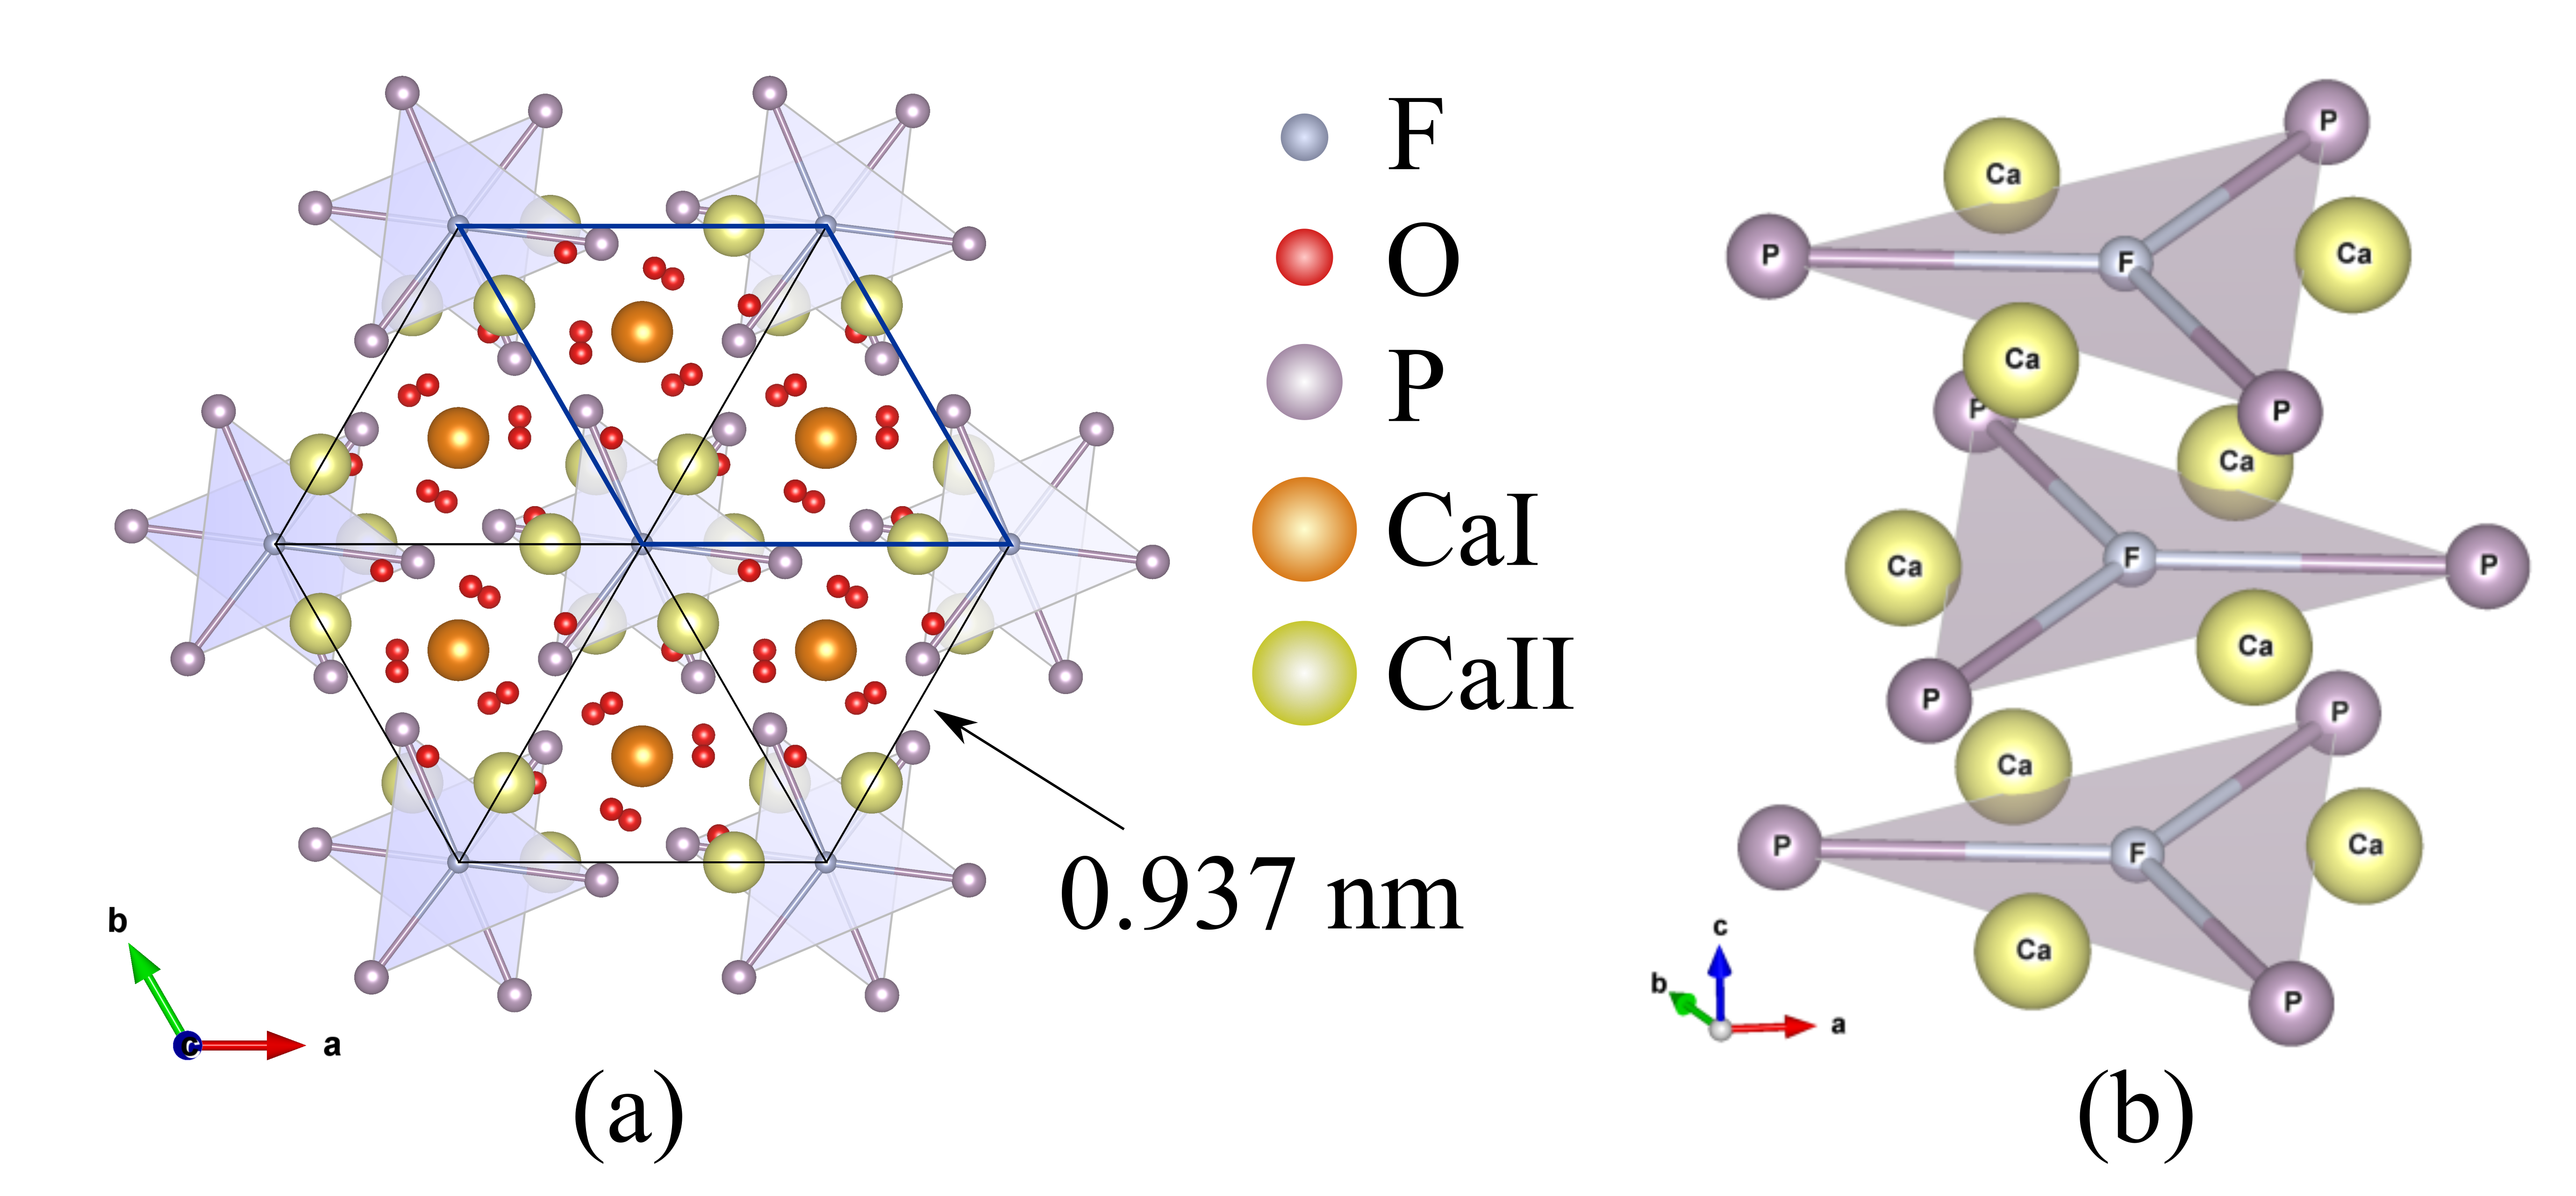
\includegraphics[width=\linewidth]{sample-fap-crystal-structure.png}
  \caption{
    (a) Структура фтористого апатита, $c$-ось направлена перпендикулярно плоскости рисунка.
    Выделена одна ячейка.
    Каждая цепь ядер $^{19}$F, идущая вдоль оси $c$, окружена шестью идентичными цепями на расстоянии $a=9.37$~\r{A}.
    (b) Часть кристаллической структуры FAp, показывающая окружение атомов фтора. Атомы кислорода были удалены для упрощения.
    Атомы фтора равномерно разнесены ($r_{FF}=344$~пкм) и расположены в колонны вдоль $c$-оси кристалла.
    Каждый атом фтора окружен тремя равноудаленными атомами фосфора при $r_{FP}=3,67$~\r{A},
    которые расположены в вершинах равносторонних треугольников на плоскости,
    перпендикулярной к $c$-оси, а также тремя ионами CaII на расстоянии 2.34~\r{A}.
  }
  \label{fig:sample-fap-crystal-structure}
\end{figure}
Хотя первый феноменологический подход к многоквантовой динамике ЯМР был развит еще в классической работе~\cite{Baum1985},
последовательная квантовомеханическая теория в настоящее время развита преимущественно для одномерных систем~\cite{Feldman1996, Feldman1997, Doronin2000, Feldman2014}.
Теория МК динамики ЯМР в одномерных системах основана на том,
что несекулярный двухспиновый/двухквантовый гамильтониан~(\ref{eq:hmq}),
описывающий многоквантовую динамику,
является $XX$-гамильтонианом~\cite{Landau5},
который для одномерных систем в приближении взаимодействий ближайших соседей может быть точно диагонализован~\cite{Mattis1993}.
В результате многоквантовая динамика ЯМР в такой системе может быть исследована аналитически.

% AMR-2020
Одномерные цепочки ядерных спинов являются редкими объектами в твердом теле из-за дальнодействующего характера прямой магнитной дипольной связи.
Одномерность нарушается из-за взаимодействия спинов из разных цепочкек.
Такие цепочки принято называть ``квазиодномерными''.
Список квазиодномерных цепочек с прямым магнитным ДДИ,
представленных в литературе,
ограничивается цепочками в кристаллах минералов группы апатита,
такими как $^{1}$H и $^{19}$F спиновые цепочки в кристаллах гидрокси- и фторапатита~\cite{Cho1996}.
Отличительной особенностью этих структур является то,
что расстояние между соседними цепочками примерно в $2.7$ раза больше,
чем расстояние между ближайшими спинами в цепочке~\cite{Cho1996}.
Ориентируя кристалл так,
чтобы внешнее магнитное поле было направлено параллельно цепочкам,
можно добиться чтобы дипольная связь между ближайшими соседями в одной цепочке была по крайней мере в 40 раз сильнее,
чем со спинами других цепочек.
Это позволяет использовать для интерпретации экспериментальных данных модель изолированной спиновой цепочки.
Первые экспериментальные исследования многоквантовой динамики ЯМР одномерных систем были начаты в~\cite{Cho1996, Gatta2012} на монокристалле гидроксиапатита кальция $\mathrm{Ca}_5(\mathrm{PO}_4)_3\mathrm{OH}$ с гексагональной системой гидроксильных протонов.
Другой пример квазиодномерной спиновой цепочки является довольно экзотическим,
поскольку был получен искусственно с помощью изотопной инженерии.
Линейные цепочки изотопов $^{29}$Si были получены в монокристалле кремния, состоящем из бесспинового изотопа $^{28}$Si~\cite{Itoh2005}.

Структура FAp, изученная с помощью рентгеноструктурного анализа \cite{Elliott1994}, изображена на Рис.~\ref{fig:sample-fap-crystal-structure} (изображения были получены с помощью программного обеспечения VESTA \cite{vesta}).
FAp представляет собой гексагональный кристалл с пространственной группой P63/m
и имеет параметры решетки $a=9.367(1)$~\r{A} и $c=6.884(1)$~\r{A}
(гексагональная ось) с одной формальной единицей Ca$_{10}$(PO$_4$)$_6$F$_2$ на каждую элементарную ячейку.
Таким образом, элементарной ячейке имеется семь кристаллографически неэквивалентных атомных центров (Рис.~\ref{fig:sample-fap-coherences}a).
Ядра $^{19}$F упорядоченны в линейную цепочку вдоль оси $c$ на гранях элементарных ячеек (Рис.~\ref{fig:sample-fap-coherences}a и b). Эти ядра разделены 1/2 размера решетки (3.44~\r{A}) на позициях z=1/4 и 3/4. При повороте на угол кратный $\pi/3$ углы элементарной ячейки совпадут с шестью ближайшими атомами F$^-$ на расстоянии 9.37~\r{A}   в плоскости перпендикулярной оси $c$. Известно, что в структуре FAp присутствует два изотопа кальция: четыре CaI и шесть CaII. Колонки Ca$^{2+}$ ионов параллельны цепочке ядер F и разделены половиной параметра решетки вдоль $c$-оси. Это 2/5 всех Ca$^{2+}$ ионов в кристалле, и они представлены изотопом CaI. Остальные узлы Ca$^{2+}$, представленные как CaII, расположены в вершинах равносторонних треугольников в плоскости, перпендикулярной $c$-оси. В центрах треугольников располагаются ионы F$^-$. Расстояние межу CaII и ионами F$^-$ 2.34~\r{A}  . Два треугольника повернуты на $60^\circ$ относительно друг друга вокруг $c$-оси. PO$_4^{3-}$ тетраэдры слегка искажены. Это приводит к трем неэквивалентным узлам кислорода. P можно представить в вершинах равносторонних треугольников, расположенных в шахматном порядке вдоль оси $c$, в плоскости, перпендикулярной оси $c$ в положениях z = 1/4 и 3/4 с ионами F$^-$ в центре (Рис.~\ref{fig:sample-fap-coherences}a). Расстояние между F и ближайшими P-ядрами составляет 3.67~\r{A}

% JETP-Lett 2015
В работах [11–14] была разработана теория МК динамики для одномерной цепочки спинов,
связанных диполь-дипольным взаимодействием,
в приближении взаимодействий ближайших соседей.
Было показано,
что в одномерной спиновой цепочке,
первоначально приготовленной в термодинамическом равновесном состоянии,
на подготовительном периоде МК ЯМР эксперимента~\cite{Baum1985},
возникают многоквантовые когерентности только нулевого и плюс/минус второго порядков.
%
Теоретические значения интенсивностей многоквантовых когерентностей ЯМР нулевого $G_0(\tau)$ и плюс/минус второго $G_{\pm2}(\tau)$ порядков
в случае длинных линейных спиновых цепей (с числом спинов $N \gg 1$) определяются формулами
%
\begin{equation}
    \label{eq:coher_g0}
    G_{0}(\tau) = \frac 1 2 + \frac 1 2 J_{0}(4D\tau)
\end{equation}
%
\begin{equation}
    \label{eq:coher_g2}
    G_{\pm2}(\tau) = \frac 1 4 - \frac 1 4 J_{0}(4D\tau),
\end{equation}
где $\tau$ - продолжительность подготовительного периода,
$D = D_{i, i+1}$ – дипольная константа связи ближайших соседей,
а $J_0$ – функция Бесселя первого рода порядка 0.
% Решение верно на относительно небольших временах подготовительного периода.

\begin{figure}[H]
  \centering
  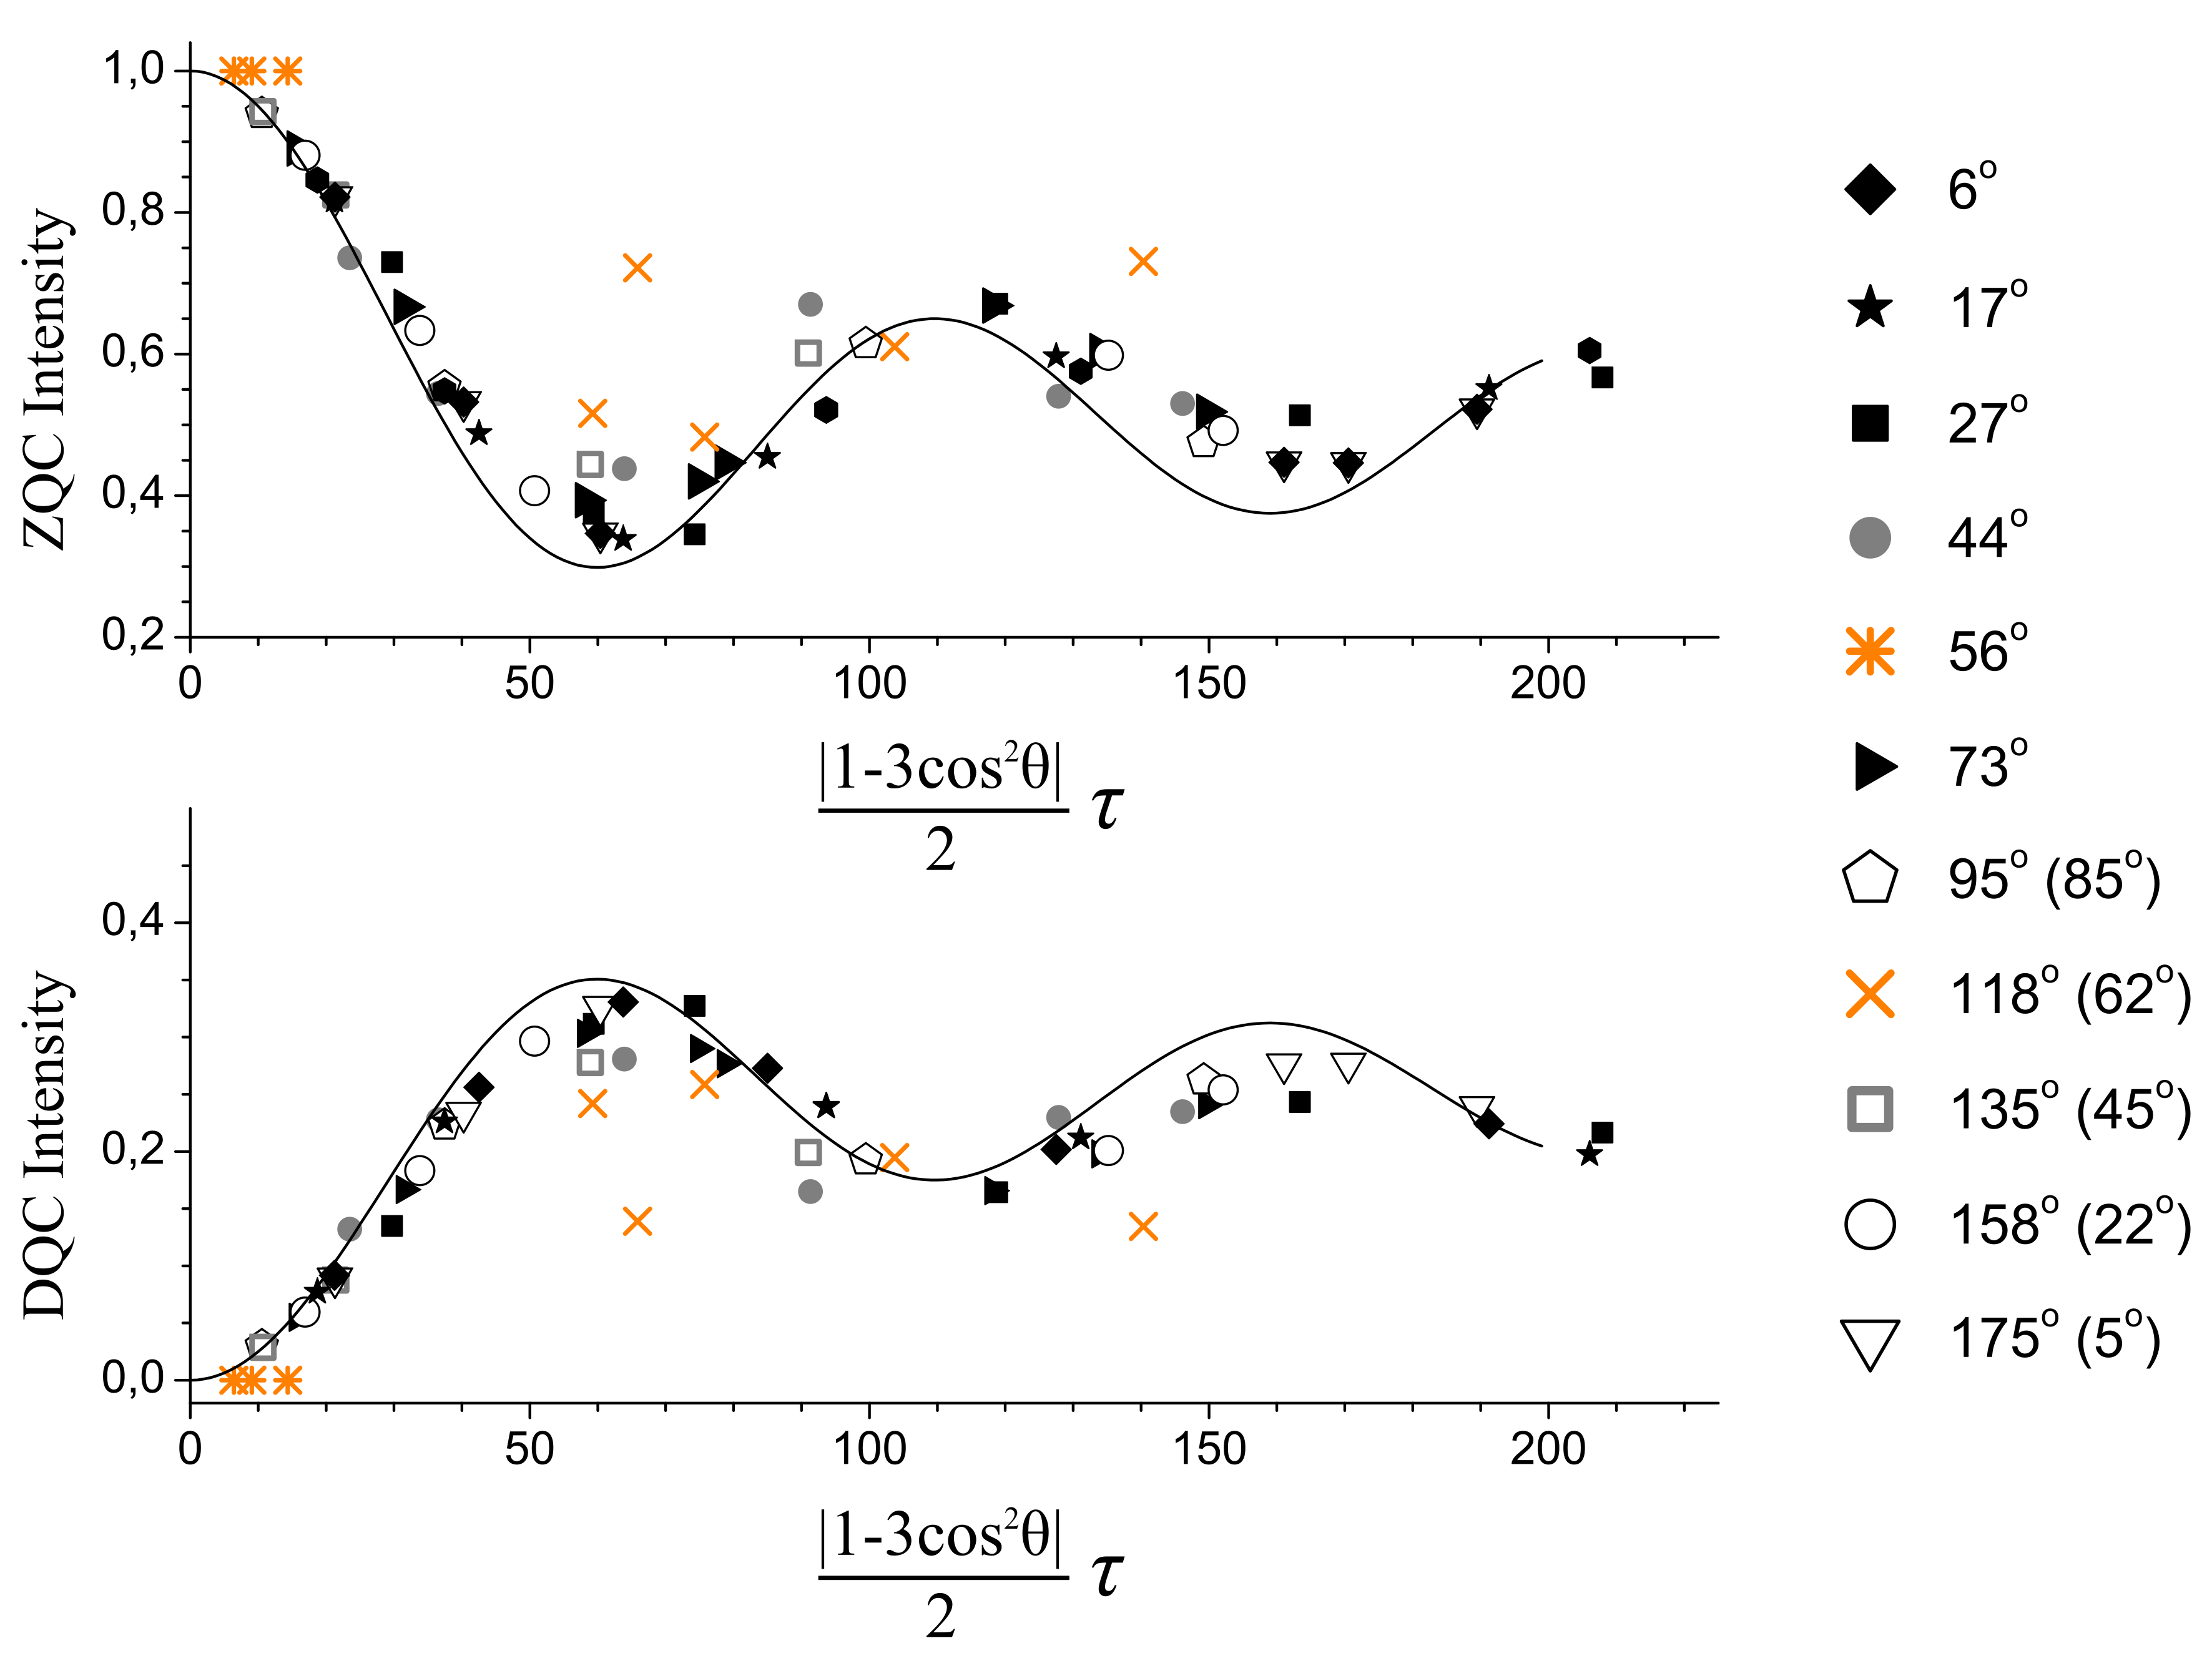
\includegraphics[width=\textwidth]{sample-fap-coherences.png}
  \caption{
    Зависимости интенсивностей МК ЯМР когерентностей нулевого $G_0(\tau)$ (сверху) и плюс/минус второго $G_{\pm2}(\tau)$ (снизу) порядков
    от масштабируемой длительности~$\bar\tau$ подготовительного периода для различных ориентаций образцов.
    Экспериментальные значения показаны в виде точек,
    a соответствующие теоретические (Ур.~(\ref{eq:coher_g0})~и~(\ref{eq:coher_g2})) результаты показаны сплошными линиями.
  }
  \label{fig:sample-fap-coherences}
\end{figure}

Принимая во внимание, что единственный аргумент, влияющий на эволюцию МК когерентности в уравнениях~(\ref{eq:coher_g0})~(\ref{eq:coher_g2}) равен $4D\tau$,
зависимость интенсивностей МК когерентности от периода подготовки для различной ориентации спиновой цепи можно обобщить простым способом\cite{Bochkin2019jmr},
введя безразмерный масштабный коэффициент $|D(\theta)/D (0)|$ для длительности подготовительного периода $\tau$.
Другими словами, можно ввести масштабированную ось длительности подготовительного периода:
%
\begin{equation}\label{eq:scaled-tau}
 \bar\tau = \left| \dfrac{1 - 3\cos^2{\theta}}{2} \tau \right|,
\end{equation}
%
для которой интенсивности МК когерентностей нулевого и плюс/минус второго порядков,
полученные при различных ориентациях,
коллапсируют на единую заданную кривую $G_0(\tau)$ и $G_{\pm 2}(\tau)$ соответственно (Рис.~\ref{fig:sample-fap-coherences}).
Абсолютное значение в выражении~(\ref{eq:scaled-tau}) объясняется тем фактом,
что интенсивности МК когерентности нечувствительны к знаку константы дипольной связи,
согласно уравнениям~(\ref{eq:coher_g0})~и~(\ref{eq:coher_g2}).

Экспериментально наблюдаемые интенсивности МК когерентностей ЯМР достаточно хорошо следуют теоретическим предсказаниям
в рассматриваемом диапазоне длительностей подготовительного периода.
Очевидные отклонения на Рис.~\ref{fig:sample-fap-coherences}) наблюдаются только для ориентаций,
близких к магическим углам ($56^\circ$ и $118^\circ$,
где дипольная связь между спинами в одной цепи становится слабой.
Для ориентации $56^\circ$ появление когерентностей порядка $\pm2$ не наблюдается.
МК когерентности  ЯМР для ориентации $118^\circ$,
по-видимому, обусловлены взаимодействиями спинов в разных цепях и, следовательно, не следуют общей тенденции.
Некоторые небольшие отклонения наблюдаются для углов $44^\circ$ и $135^\circ$,
которые все еще близки к магическому углу.
Последние отклонения можно отнести к большему влиянию погрешности установки угла.
Изменения дипольной константы в этом диапазоне являются самыми сильными,
что приводит к большей ошибке в определении поправочного коэффициента для времени подготовки.
Ориентации цепи, близкие к перпендикулярному внешнему магнитному полю,
не показывают существенных отклонений МК интенсивностей несмотря на то,
что внутрицепочечное дипольное взаимодействие уменьшается примерно в два раза,
а константа межцепочечного взаимодействия максимальна.
Учитывая, что единственным регулируемым параметром в теории является дипольная константа связи,
между ближайшими соседями в цепи, данные очень хорошо соответствуют кривой.


% mrjs-2019
% JETP-2018

% \begin{figure}
%   \centering
%     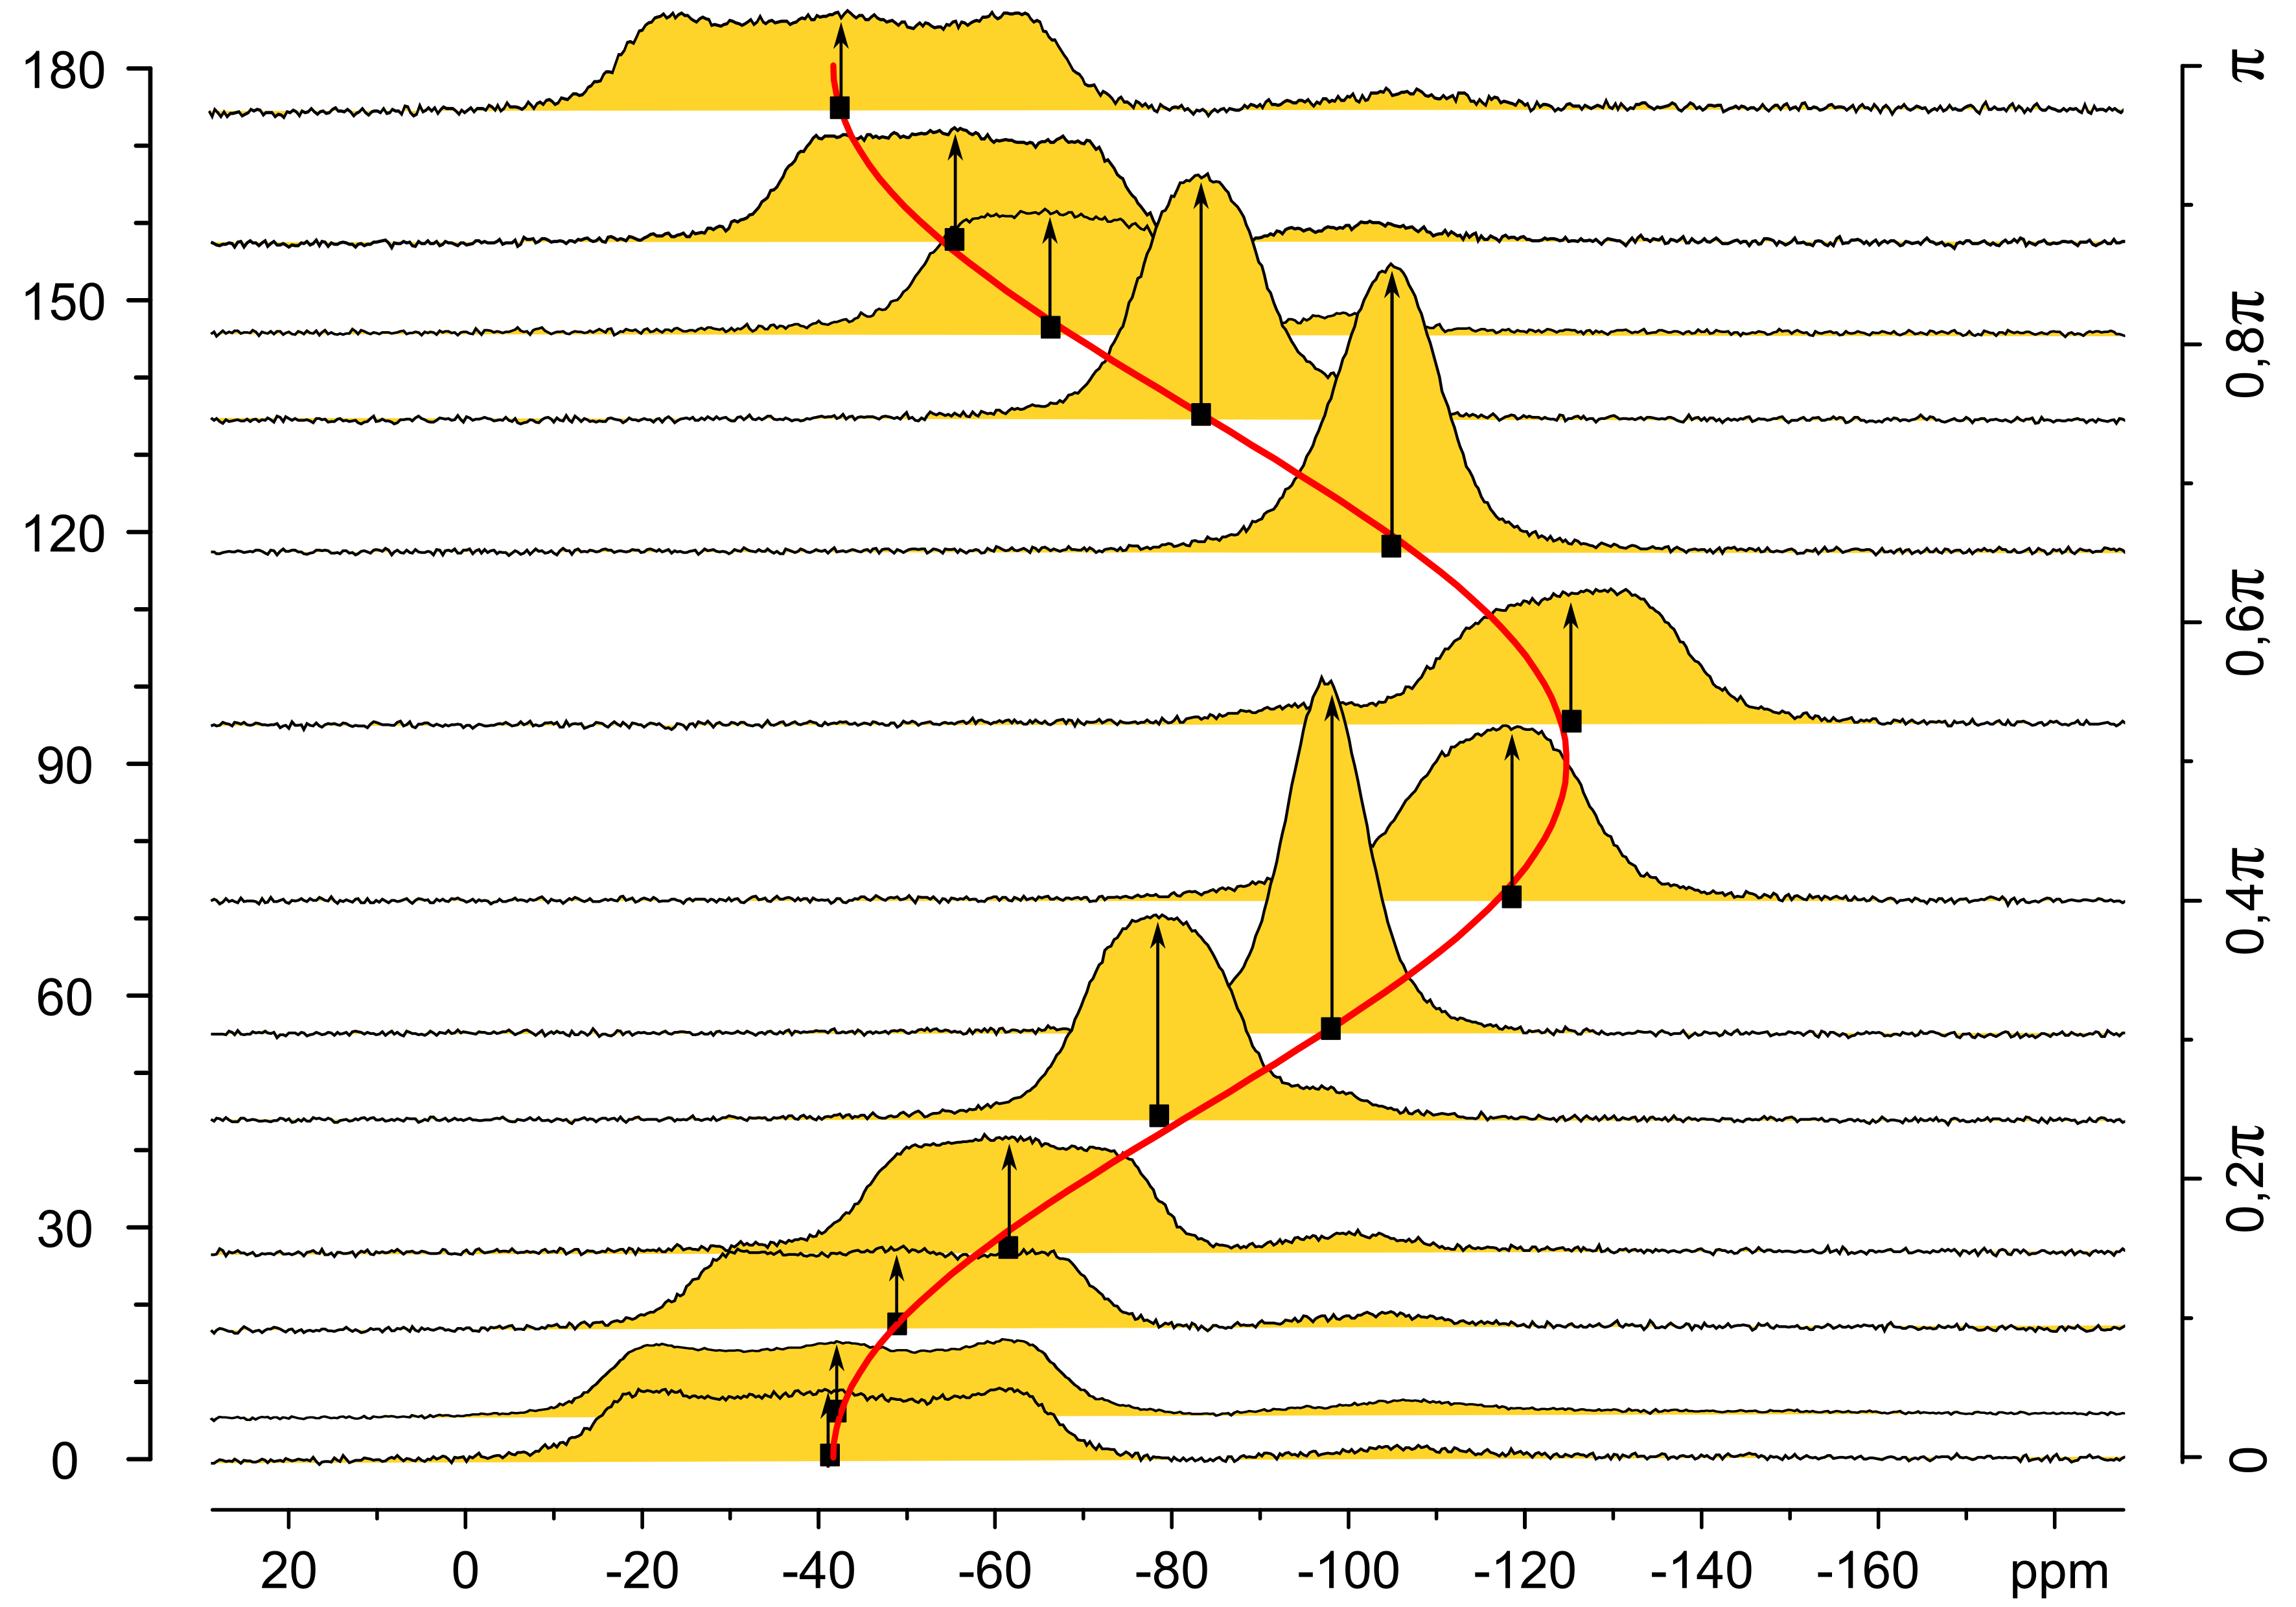
\includegraphics{sample-fap-nmr-spectrum.png}
%     \caption{Изменение $^19$F ЯМР спектра фтористого апатита во время вращения $c$-оси кристалла вокруг оси перпендикулярной направлению внешнему магнитного поля}
%   \label{fig:my_label}
% \end{figure}

\subsection{Зигзагобразная цепочка ядерных спинов}
\label{sec:model-zigzag-chain}
% JMR-2020 G.A. Bochkin and et al., \textit{J. Magn. Res.} \textbf{319}, 106816, (2020)
% AMR-2020

\begin{figure}
  \centering
  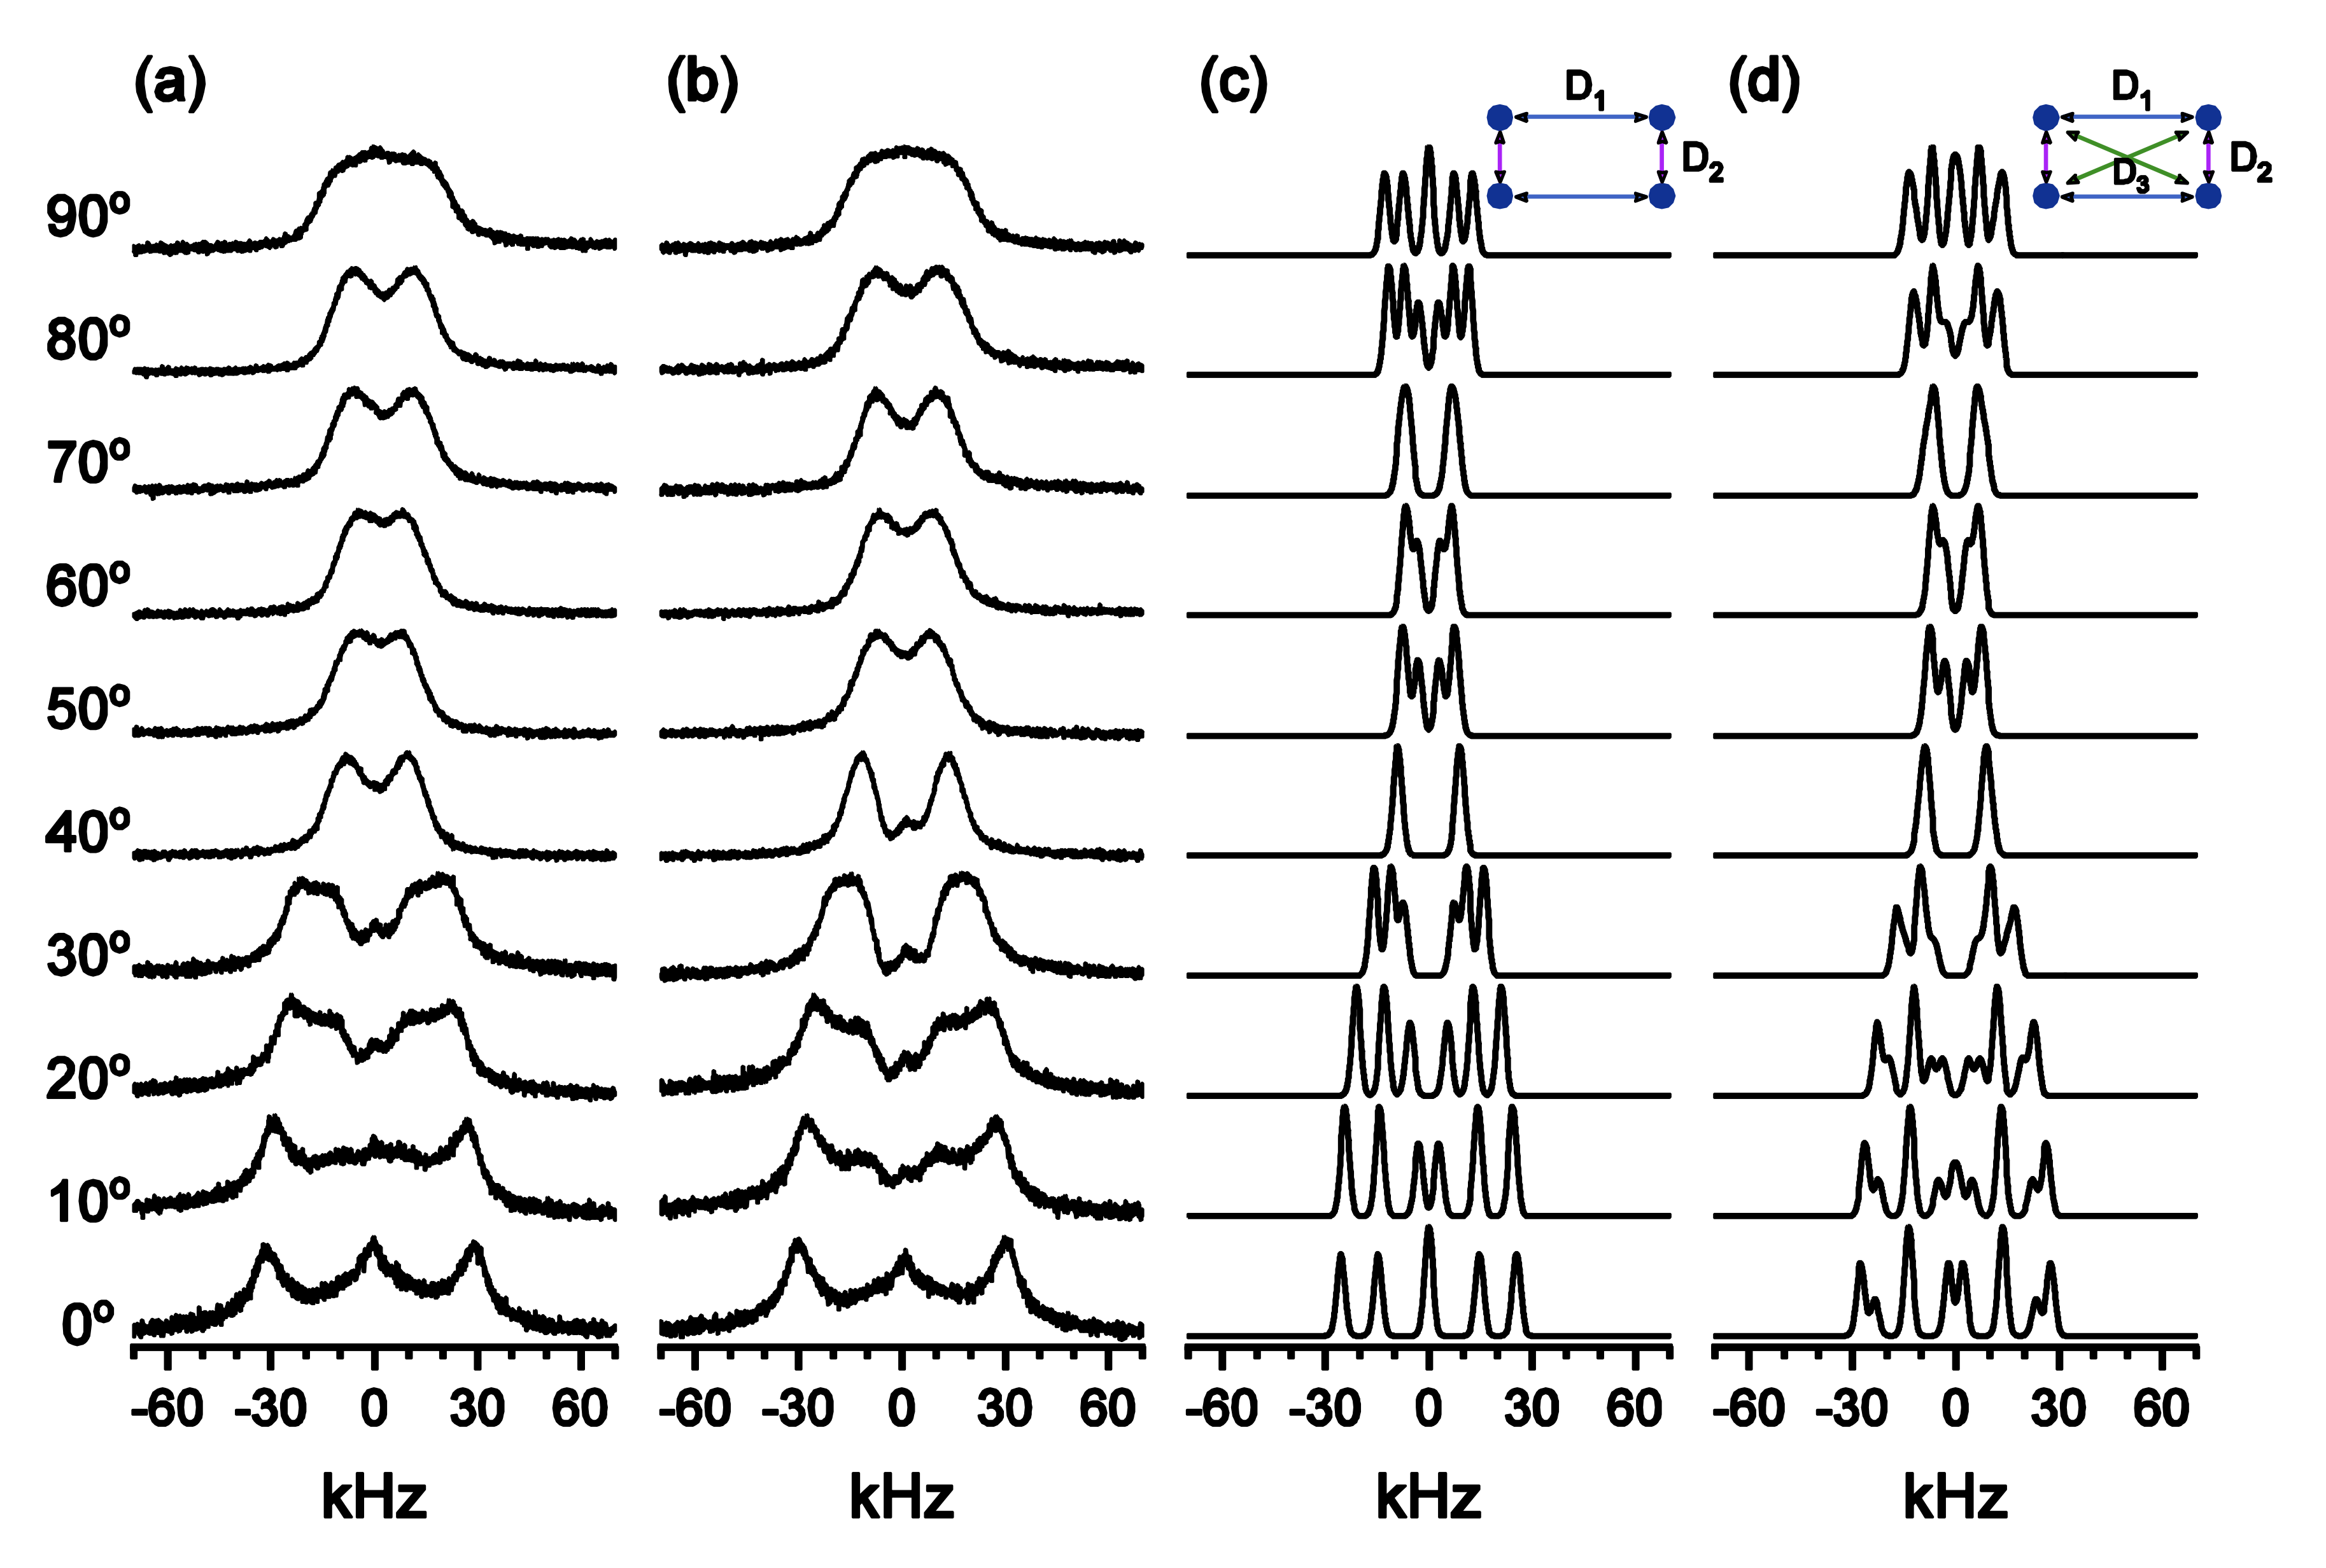
\includegraphics[width=\textwidth]{sample-hambergite-nmr-spectrum.png}
  \caption{
    Спектры ЯМР протонов $^1$H монокристалла гамбергита при вращении в двух различных плоскостях.
    Ось ординат --- это угол между осью цепи ($c$-ось кристалла) и внешним магнитным полем.
    Экспериментальные данные в случае, когда
    ось вращения перпендикулярна $c$-оси и параллельна плоской плоскости кристалла,
    и когда перпендикулярна $c$-оси и плоской плоскости,
    изображены на (a) и (b) соответственно.
    Теоретические спектры для модельной цепочки,
    состоящей из четырех спинов, соединенных в кольцо (прямоугольник),
    с учетом только ближайших соседей и включая соседние взаимодействия,
    изображены на (c) и (d) соответственно.
  }
  \label{fig:sample-hambergite-nmr-spectrum}
\end{figure}

\begin{figure}
  \centering
  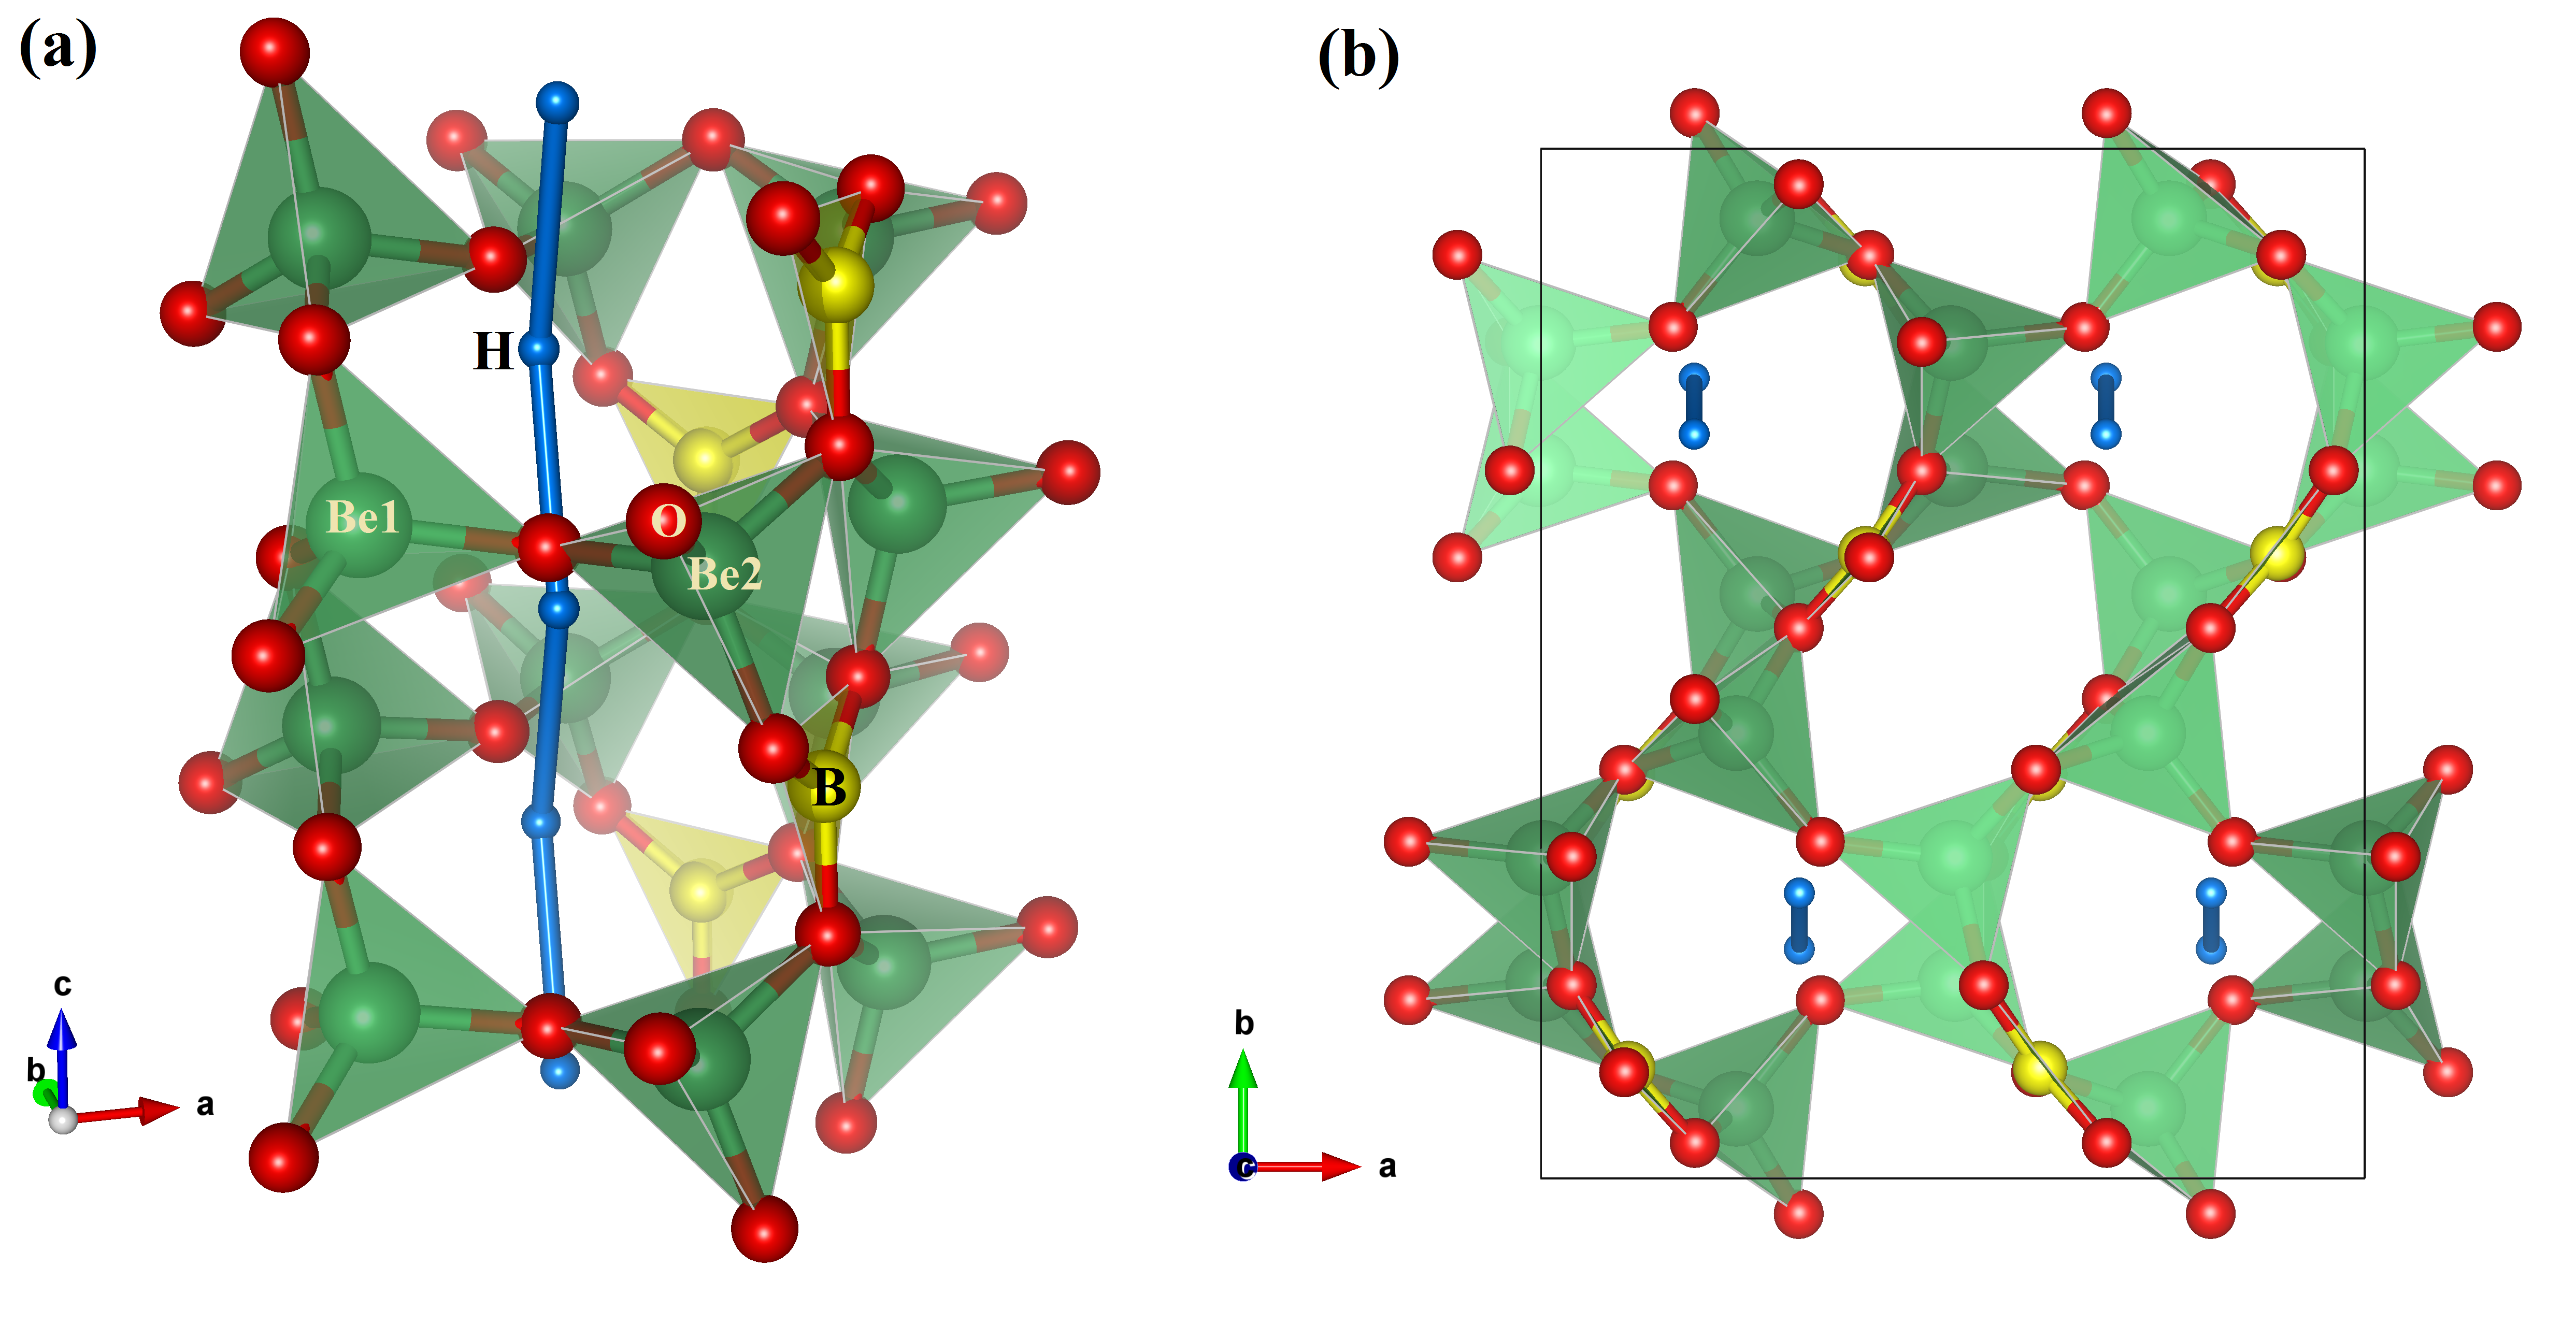
\includegraphics[width=\textwidth]{sample-hambergite-structure.png}
  \caption{
    Структура гамбергита $\mathrm{Be}_2\mathrm{BO}_3(\mathrm{OH})$.
    (a) Цепочка протонов и соседние атомы.
    (b) Вид вдоль кристаллографической $c$-оси.
  }
  \label{fig:sample-hambergite-structure}
\end{figure}
% AMR-2020
В этом разделе будет рассмотрена экзотическая модель спиновой цепочки с чередующейся дипольной связью.
До сих пор данная структура не была исследована в МК эксперименте ЯМР.
Примером такой спиновой модели является квазиодномерная цепочка гидроксильных протонов в кристаллах гамбергита $\mathrm{Be}_2\mathrm{BO}_3(\mathrm{OH})$~\cite{Zachariasen1931, Gatta2012}.
Химический состав и кристаллическая структура гамбергита существенно отличаются от структуры апатита.
На первый взгляд, эти различия не в пользу гамбергита,
если рассматривать его как спиновую цепочку.
Относительная плотность ядер, составляющих цепочку (ядра $^1$Н),
в гамбергите значительно больше, чем в апатите (ядра $^{19}$F или $^1$Н).
Вследствие этого изолируемость отдельных спиновых цепочек хуже.
Количество других ядер,
обладающих значительным магнитным   моментом,
в гамбергите также больше.
Тем не менее гамбергит демонстрирует тонкую структуру спектров ЯМР $^1$Н (Рис.~\ref{fig:sample-hambergite-nmr-spectrum}),
характерную для одномерных цепочек.
Расчеты второго момента $^1$Н Ван Флека в работе~\cite{Bochkin2020jmr} показывают,
что основной вклад вносят спины в одной цепи,
что сравнимо со случаем апатита.
Особенностью $^1$Н спиновых цепочек гамбергита является то,
что спины в них расположены не вдоль прямой линии,
как в случае апатита,
а образуют зигзаг вдоль направления цепочки (Рис.~\ref{fig:sample-hambergite-structure}).
Таким образом, в зависимости от ориентации во внешнем магнитном поле,
цепочка может рассматриваться как однородная,
с равными дипольными константами среди всех пар ближайших спинов,
или зигзагообразная,
где дипольная связь между ближайшими соседями чередуется между двумя значениями для последовательных пар спинов.

Гамбергит представляет собой орторомбический кристалл с пространственной группой Pbca
и параметрами решетки a = 9,762(2)~\r{A}, b = 12,201(2)~\r{A} и c = 4,430(1)~\r{A}~\cite{Gatta2012}.
Число структурных единиц в элементарной ячейке равно Z = 8.
Кристаллическая структура гамбергита показана на Рис.~\ref{fig:sample-hambergite-structure}.
Структура кристалла гамбергита может быть описана~\cite{Zachariasen1931, Zachariasen1963, Gatta2012, Burns1995} как состоящая из двух различных строительных блоков:
$\mathrm{BeO}_3(\mathrm{OH})$ тетраэдров
и $\mathrm{BO}_3$ треугольников.
Имеются две различные позиции Be,
каждая из которых координируется тремя атомами O и группой OH.
Каждый негидроксильный атом кислорода в тетраэдрах $\mathrm{BeO}_3(\mathrm{OH})$
разделяется с другой единицей $\mathrm{BeO}_3(\mathrm{OH})$
и треугольником $\mathrm{BO}_3$.
Боратная группа существует в виде почти идеального кислородного треугольника с атомом бора в центре.
Группа OH разделяется между двумя тетраэдрами $\mathrm{BeO}_3(\mathrm{OH})$,
а треугольники $\mathrm{BO}_3$ лежат в плоскости, параллельной оси $c$.
Такое межполиэдрическое соединение приводит к каркасоподобной структуре с искаженными каналами,
идущими вдоль $c$-оси.
Один из двух видов каналов содержит зигзагообразные цепочки спинов $^1$H.
Эти цепочки лежат в плоскостях, параллельных $bc$-плоскости.

\begin{table}[h]
  \centering
  \begin{tabular}{|c|c|c|c|}
    \hline
    Изотоп & Природное содержание, \% & Гиромагнитное отношение, $\frac{\mbox{рад}}{c \cdot T}$ & Спин \\ %  рад с$^{-1}$ Т$^{-1}$
    \hline\hline
    $^9$Be & 100 & $3,75966 \times 10^7$ & 3/2 \\
    \hline
    $^{10}$B & 19,9 & $2.87468 \times 10^7$ & 3 \\
    \hline
    $^{11}$B & 81,1 & $8.584707 \times 10^7$ & 3/2 \\
    \hline
  \end{tabular}
  \caption{
    ЯМР-активным ядра в структуре гамбергита.
   }
  \label{tab:hambergite-isotopes}
\end{table}

Оценим применимость модели одномерных спиновых цепочек для кристалла гамбергита,
на основе атомных координат, предоставленных Гатта и др.~\cite{Gatta2012}.
Проведем сравнение со структурой фторапатита,
который, как известно,
является хорошей моделью одномерной цепи в широком диапазоне ориентаций во внешнем магнитном поле~\cite{Bochkin2019}.
Ячейки фторапатита и гамбергита сравнимы по размеру (объемы $526.0$~\r{A}$^3$ и $527.6$~\r{A}$^3$, соответственно),
но последний содержит в 4 раза больше протонов
(каждая ячейка содержит 8 протонов, принадлежащих 4 цепочкам).
Расстояние между ближайшими протонами в гамбергите составляет $2.312$~\r{A}.
Угол между ближайшими соседями и направлением цепи постоянен и составляет приблизительно $16.7^\circ$.
Расстояние до ближайшего протона в соседней цепи составляет $4.940$~\r{A}.
Из этого следует, что изоляция спиновых цепей в гамбергите должна быть намного хуже, чем во фторапатите.
Действительно, ближайшие спины соседних цепочек в гамбергите находятся только в $2.1$ раза дальше,
чем ближайшие спины в цепочке,
по сравнению с почти 3 разами во фторапатите.
Расстояние между ближайшими протонами в гамбергите постоянно,
но они не лежат вдоль одного направления,
в отличие от фторапатита,
где спины одинаково расположены вдоль $c$-оси.
Спины в гамбергите расположены цепочками вдоль $c$-оси зигзагообразно.
Плоскости цепочек параллельны $bc$-плоскости  (см. Рис.~\ref{fig:sample-hambergite-structure}).
Ближайшие соседи в цепочке лежат строго вдоль $c$-оси кристалла
и расстояние между ними равно параметру латентности $c = 4.43$~\r{A}.
Расстояние между плоскостями цепочки вдоль направления $a$ равно половине этого параметра $a/2 = 4.881$~\r{A}.
Расстояние между осями цепей вдоль направления $b$ приблизительно равно половине этого параметра $b/2 = 6.101$~\r{A}.
Аналогично случаю расположения спинов вдоль $c$-оси,
оси цепей вдоль направления $b$ расположены в шахматном порядке (см. Рис.~\ref{fig:sample-hambergite-structure}b и Рис.~\ref{fig:sample-hambergite-structure}c).
В орторомбической системе гамбергита две ближайшие цепи лежат в направлении $a$.
Взаимодействие с двумя ближайшими протонами в этих цепях в 17 раз меньше,
чем взаимодействие ближайших спинов в цепи.
Взаимодействие с остальными окружающими спинами по крайней мере в 30 раз слабее.
Другим важным моментом, который необходимо учитывать в структуре гамбергита,
являются гетероядерные дипольные взаимодействия,
поскольку число магнитно-активных изотопов больше по сравнению с фторапатитом.
Ядра кислорода можно смело игнорировать из-за низкой природной распространенности и низкого гиромагнитного отношения,
но остальные ядра в структуре гамбергита являются ЯМР-активными (см. Таблицу~\ref{tab:hambergite-isotopes}).
Тем не менее расчеты~\cite{Bochkin2020jmr},
учитывающие реальную геометрию и разницу в магнитных моментах,
показывают, что доминирует дипольная связь между спинами в одной цепи.
Вклад, обусловленный дипольным взаимодействием со спинами в одной цепочке, составляет более 96\% от общего второго момента,
когда цепочка ориентирована вдоль внешнего магнитного поля.
Этот вклад уменьшается до 88\% для 1H спиновых цепочек гамбергита,
наклоненных на 30 градусов от внешнего магнитного поля.
Экспериментальная форма линии ЯМР $^1$H может быть описана
с учетом взаимодействия c относительно небольшим количеством ближайших спинов в цепочке.
Полученные результаты подтверждают,
что спины $^1$H в кристаллах гамбергита могут служить хорошей моделью квазиодномерной спиновой цепи.


\subsection{Модель эквивалентных спинов}
\label{sec:model-equivalent-spins}
% J. Baugh, A. Kleinhammes, D. Han, Q. Wang, and Y. Wu, Science 294, 1505 (2001).
\begin{figure}[H]
  % \begin{subfigure}[t]{0.32\textwidth}
  %   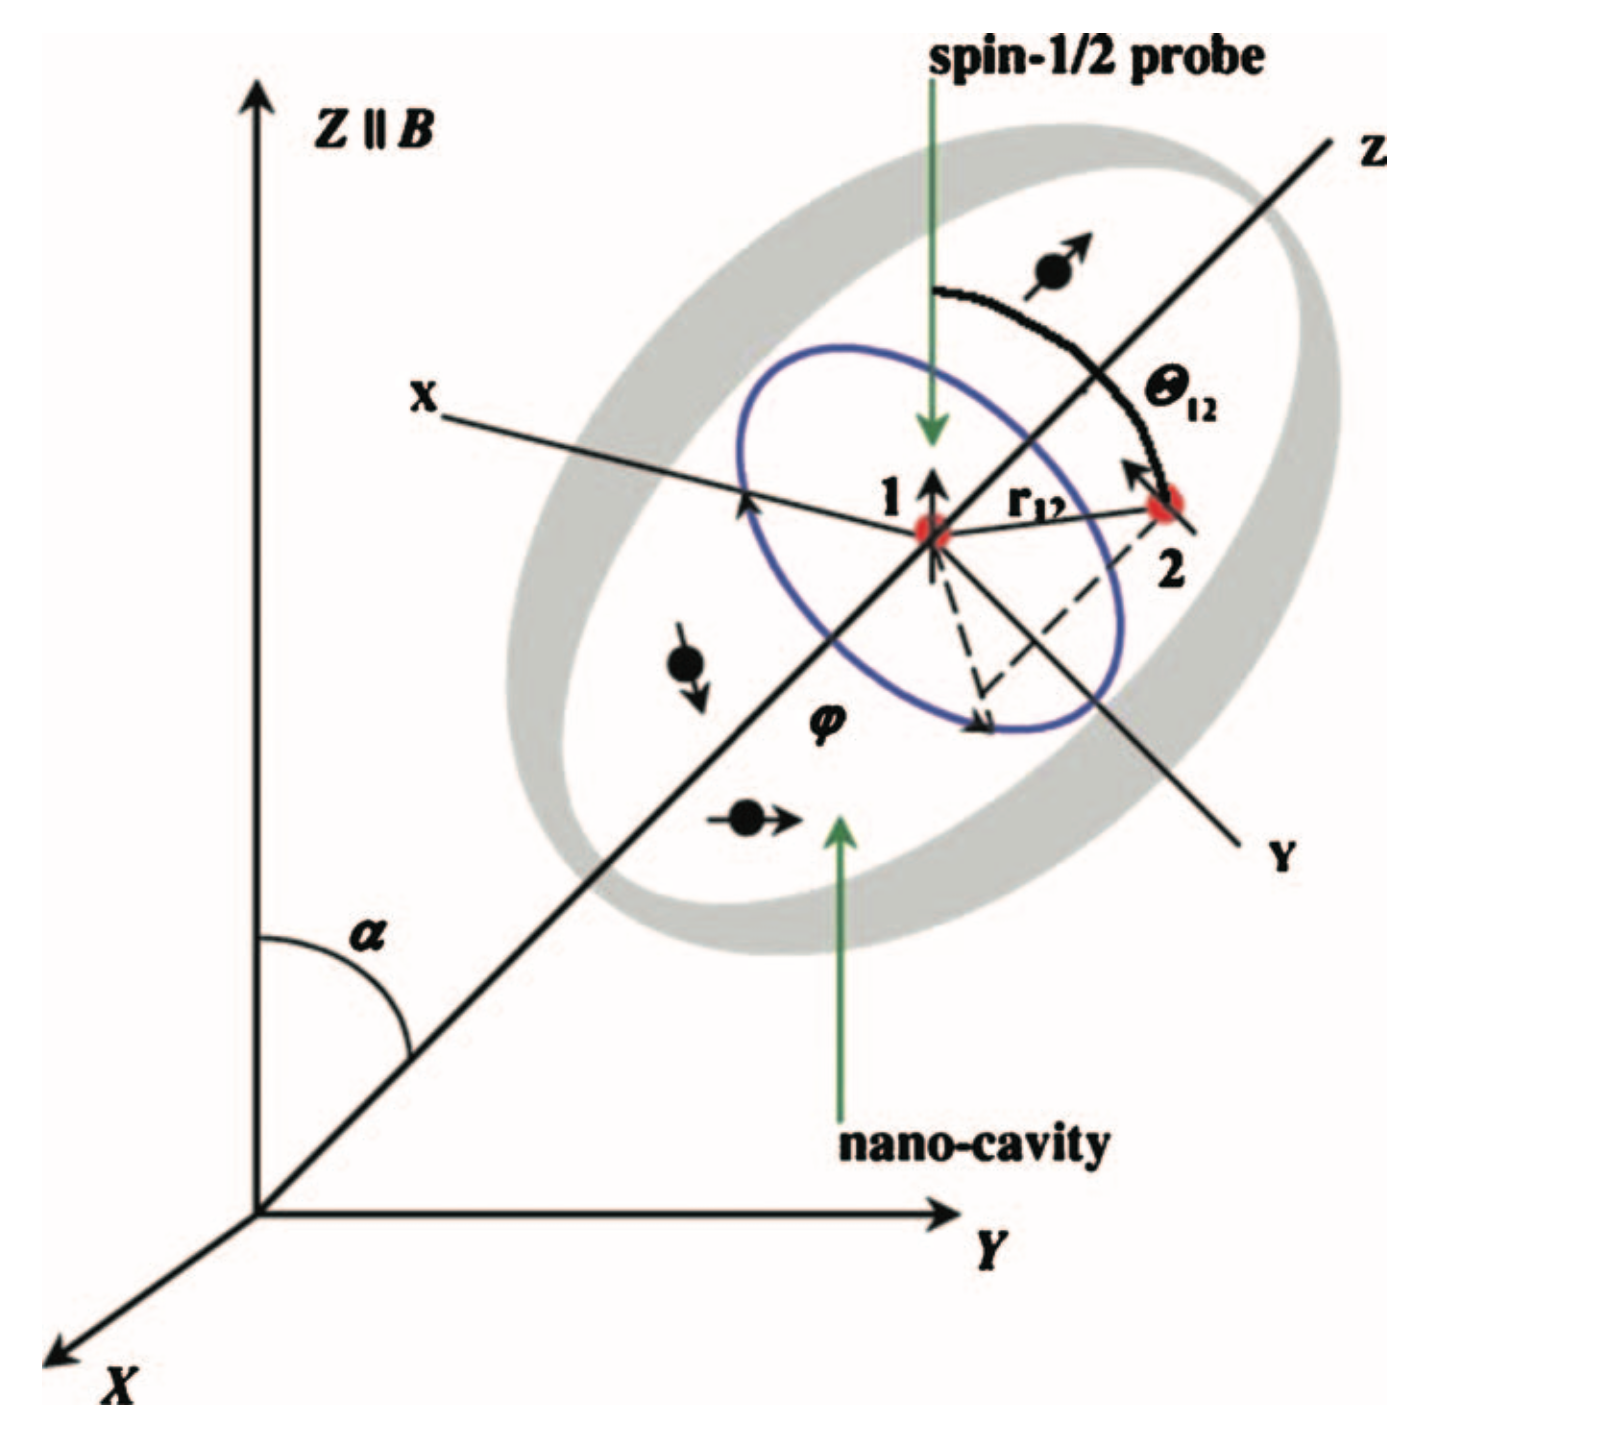
\includegraphics[width=\textwidth]{model-nanopore-schema.png}
  %   \caption{
  %     Hанопор~\cite{Baugh2001}
  %     со спин-несущих молекулами во внешнем сильном магнитном поле $\vec B$.
  %   }
  % \end{subfigure}
  % \hfill
  \begin{subfigure}[t]{0.55\textwidth}
    \centering
    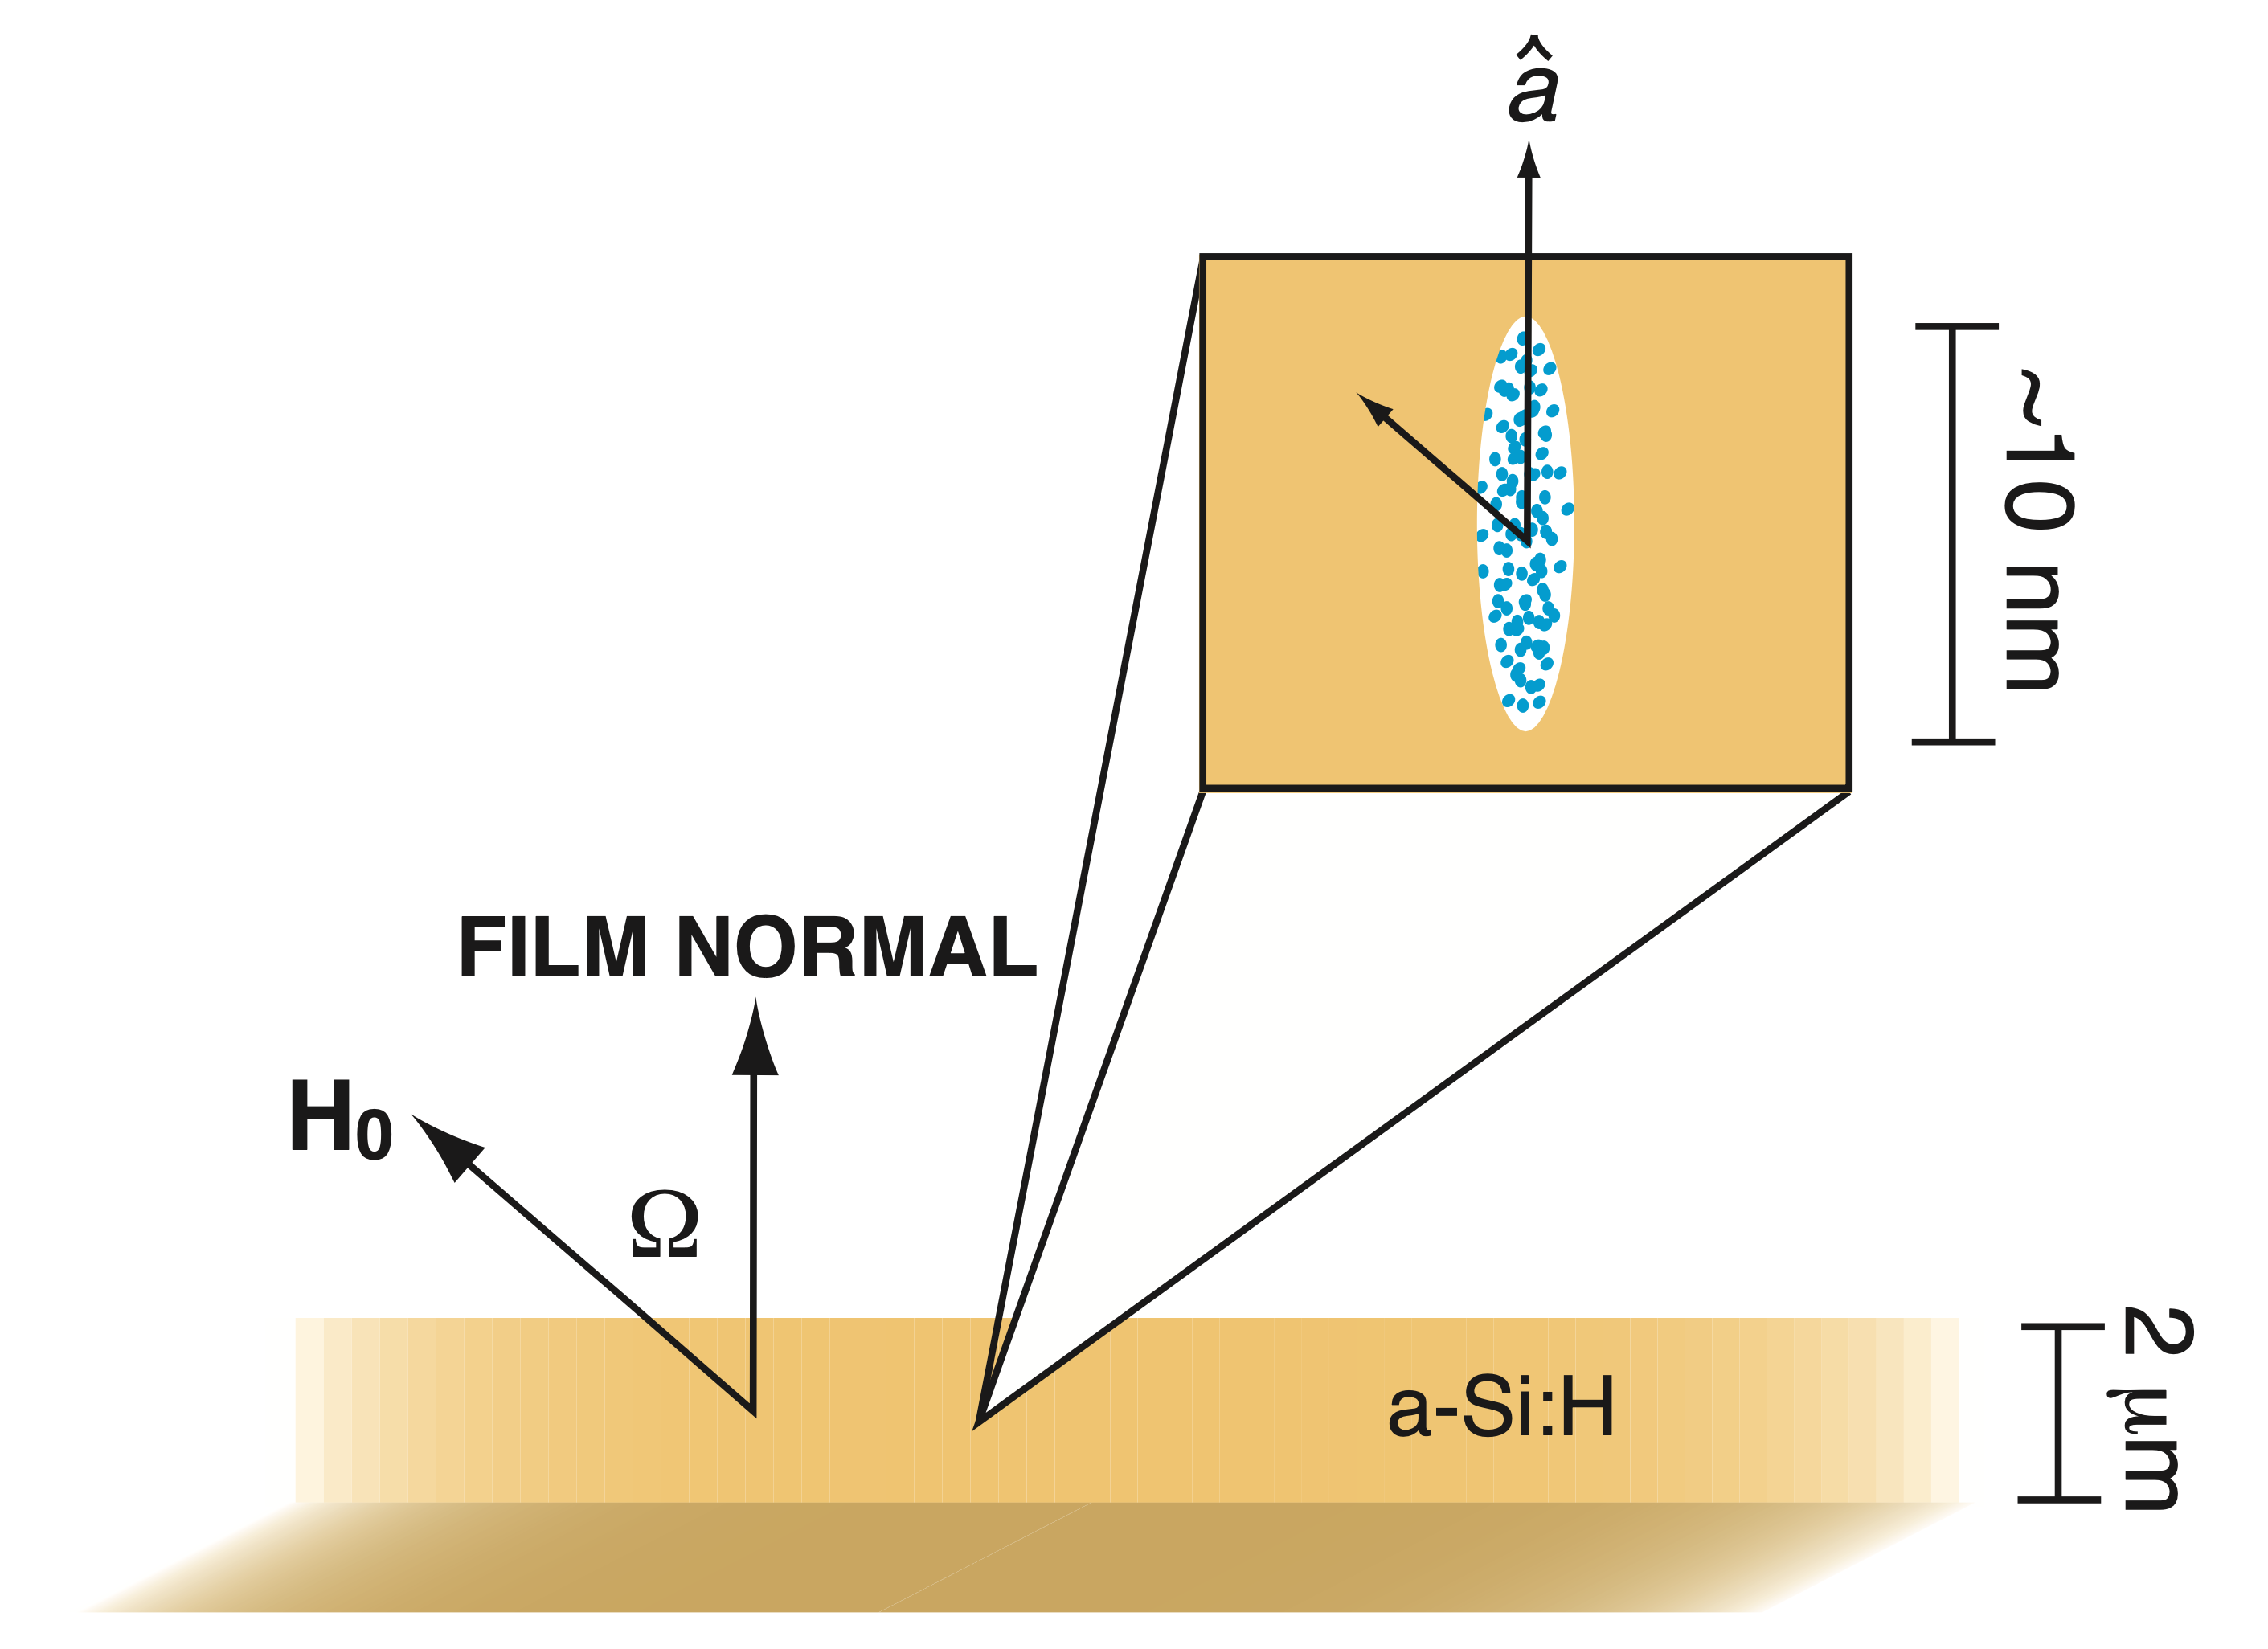
\includegraphics[width=\textwidth]{sample-nanopore-film.png}
    \caption{\protectИллюстрация поперечного сечения тонкой пленки гидрогенизированного аморфного кремния (a-Si:H) с увеличенной областью,
показывающей вытянутую нанопору,
содержащую газ H$_2$ (синие точки).
$\Omega$ --- угол между внешним магнитным полем (H$_0$) и главной осью нанопоры.
}
    \label{fig:sample-nanopore-film}
  \end{subfigure}
  \hfill
  \begin{subfigure}[t]{0.4\textwidth}
    \centering
    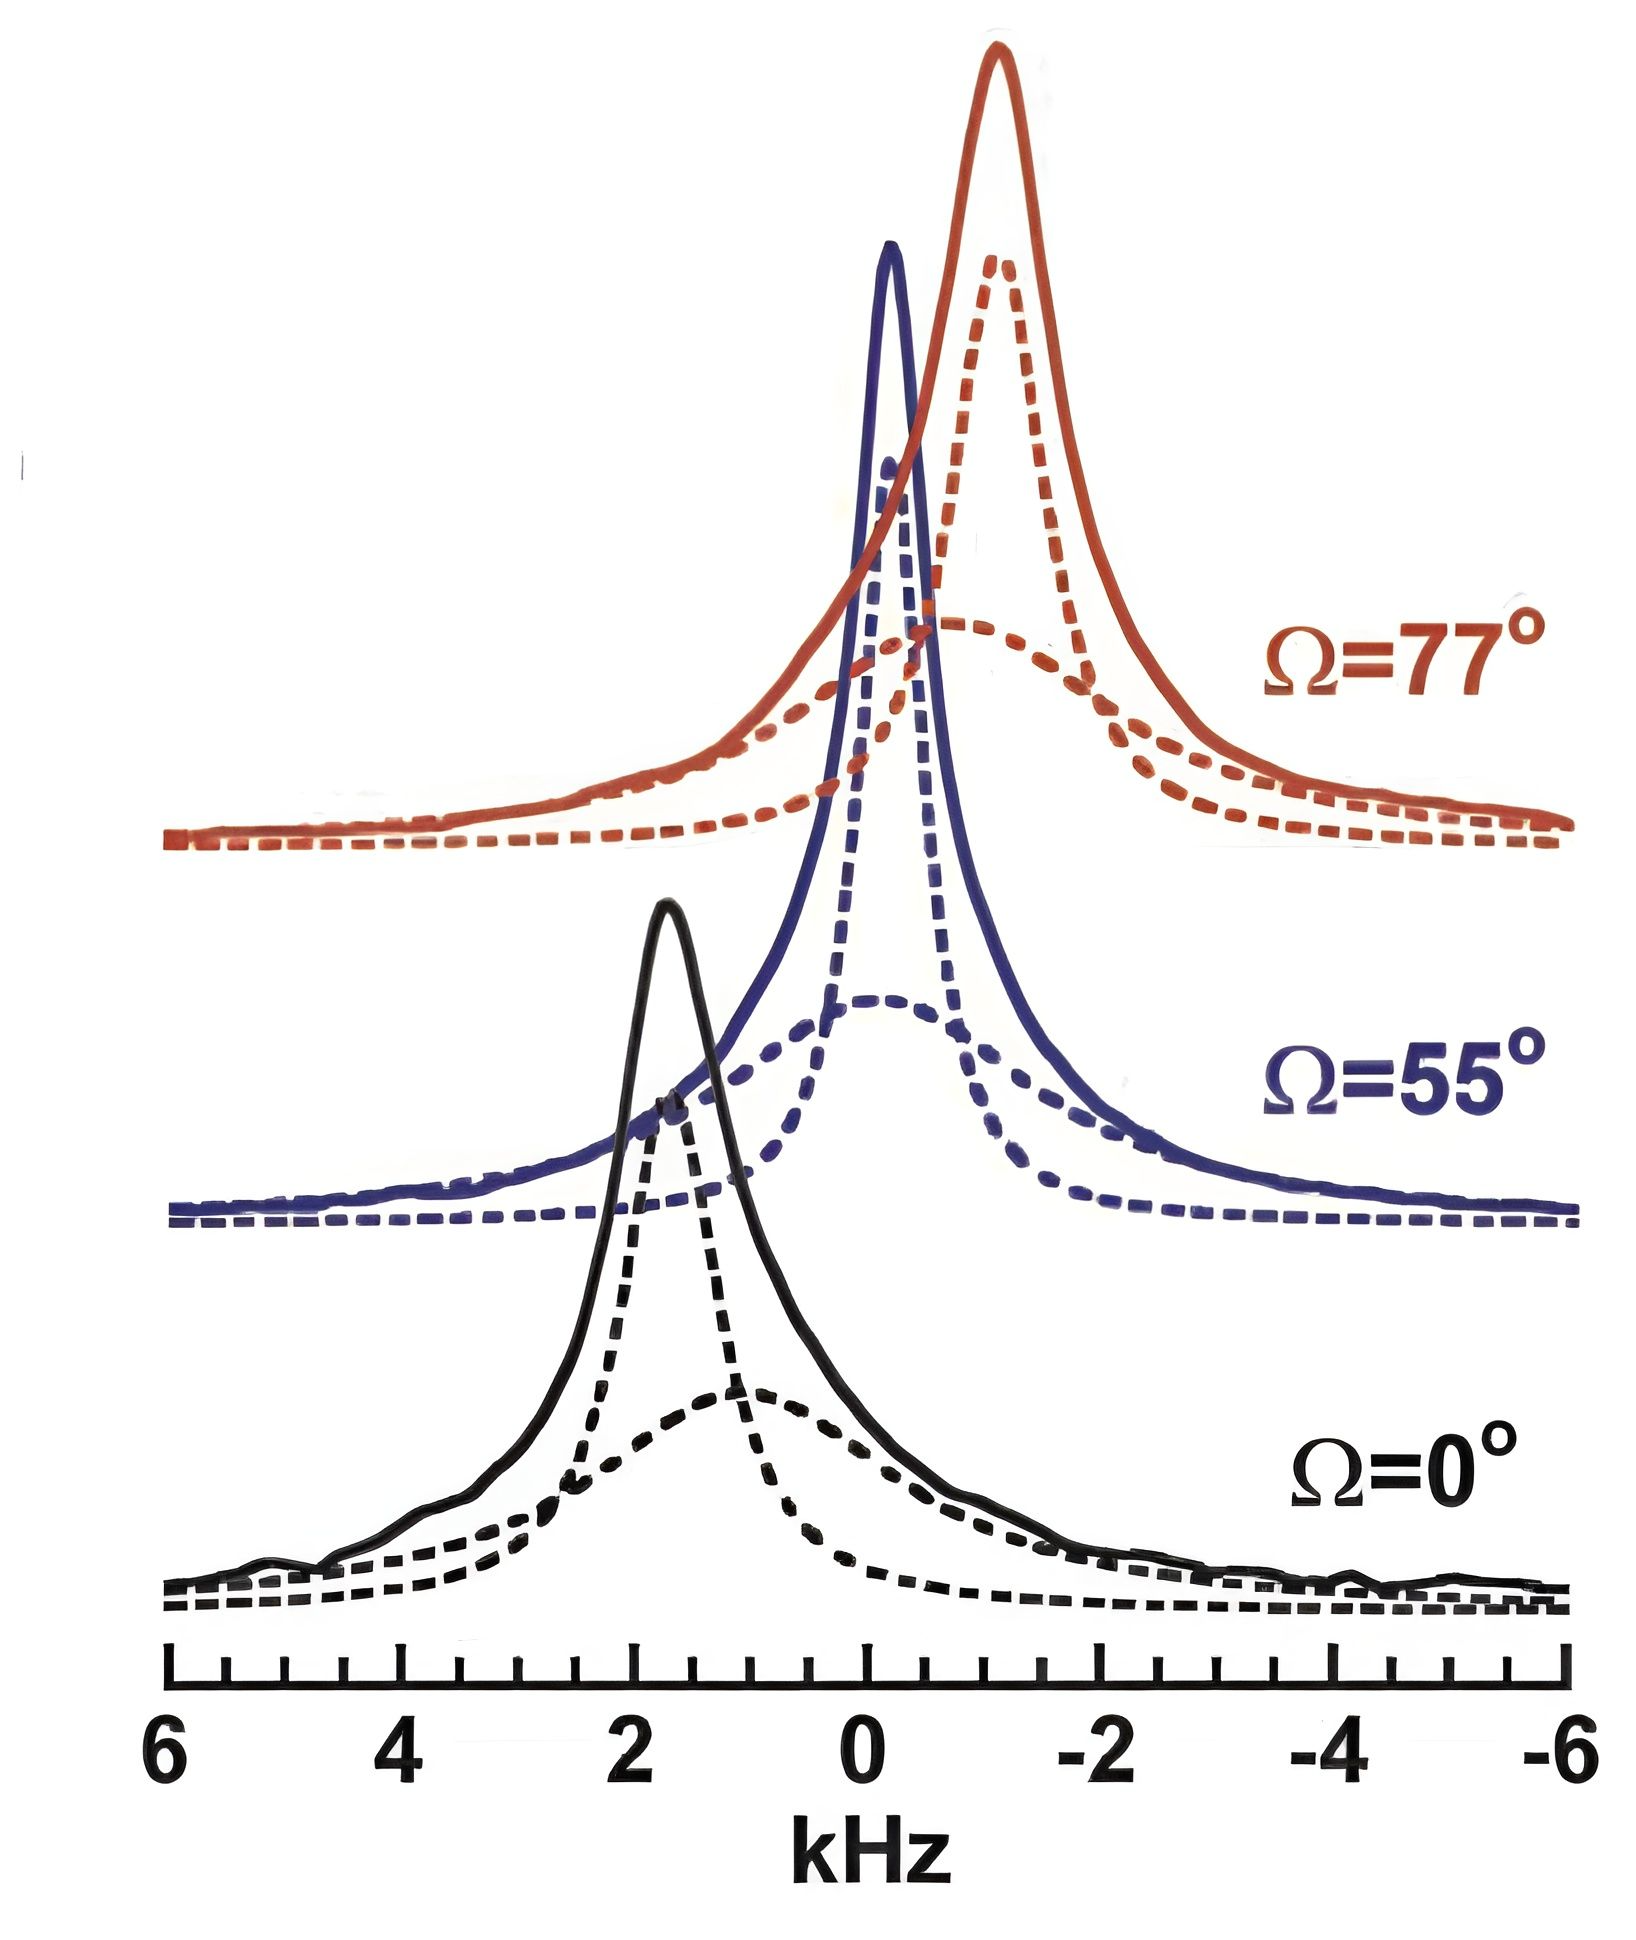
\includegraphics[width=\textwidth]{sample-nanopore-nmr-spectrum.png}
    \caption{\protectСпектры ЯМР протонов при комнатной температуре (сплошные линии)
и их линейные подгонки (пунктирные линии)
для тонкой пленки a-Si:H,
снятые при различных ориентациях пленки относительно приложенного магнитного поля (4,7 тесла).
Угол определен на  Рис.~\ref{fig:sample-nanopore-film}.
Значение константы связи $D$ зависит как от газа,
так и от эффективного давления в нанопоре ($\approx 1$ кБар).
$\Omega$ --- угол между внешним магнитным полем (H$_0$) и главной осью нанопоры.}
    \label{fig:sample-nanopore-nmr-spectrum}
  \end{subfigure}
  % \captionsetup{skip=-0.1mm}
  \caption{}
\end{figure}


%PRA-2019
Для исследования многочастичной запутанности необходима такая модель взаимодействующих спинов,
в которой многоспиновая динамика может быть изучена при низких температурах.
Важно, чтобы модель содержала достаточно большое число спинов,
и теория МК ЯМР была применима при произвольных температурах.
Только тогда можно исследовать многоспиновую запутанность и ее зависимость от температуры.
Несмотря на то, что уже разработана последовательная квантово-механическая теория МК динамики ЯМР для одномерных систем~\cite{Feldman1996, Feldman1997, Doronin2000},
они плохо подходят для исследования многочастичной запутанности.
Дело в том, что точные решения для МК динамики ЯМР в одномерных системах показывают~\cite{Feldman1996, Feldman1997, Doronin2000},
что, начиная с состояния термодинамического равновесия,
в приближении ближайших соседей возникают только нулевые и двойные квантовые когерентности.
В результате второй момент (дисперсия) МК спектра ЯМР мал, и многоквантовая запутанность не возникает.
% Doronin2009jcp
Дальние взаимодействия приводят к когерентностям более высокого порядка в МК спектрах ЯМР.
Однако эти взаимодействия находятся за пределами точных решаемых моделей~\cite{Munowitz1987, Alvarez2015, Wei2018}.
Таким образом, необходимо применять численные методы, чтобы учесть дальние спин-спиновые связи.
Тем не менее даже суперкомпьютерные расчеты позволяют изучать МК динамику ЯМР спиновой цепочки,
состоящей не более чем из двадцати пяти спинов,
что недостаточно для исследования многочастичной запутанности в рамках МК динамики ЯМР.

Для исследования многоквантовой запутанности подходит модель эквивалентных спинов.
Примером такой модели является  несферическая нанопора~\cite{Baugh2001},
заполненная газом спин-несущих атомов (например, ксеноном) (Рис.~\ref{fig:sample-nanopore-film})
или молекул в сильном внешнем магнитном поле.
Диполь-дипольные взаимодействия (ДДВ) спин-несущих атомов (молекул) в таких нанопорах не усредняются до нуля
в процессе молекулярной диффузии из-за несферичности нанопоры~\cite{Baugh2001, Feldman2004}.
Остаточные усредненные ДДВ определяются только одной константой связи (Рис.~\ref{fig:sample-nanopore-nmr-spectrum}),
которая одинакова для всех пар взаимодействующих спинов~\cite{Baugh2001, Feldman2004}.
Значение константы связи зависит как от газа,
так и от эффективного давления в нанопоре ($\approx 1$ кБар).
Это означает, что, по существу, мы имеем систему эквивалентных спинов.
Ниже будет показано, что МК динамика ЯМР такой системы может быть исследована точно~\cite{Doronin2009}.
Необходимо подчеркнуть,
что существуют некоторые ограничения для реализации описанной модели
при исследовании нанопористых соединений МК методами ЯМР.
Например, модель предполагает, что все нанопоры имеют одинаковый объем и одинаковую ``несферическую'' форму.


На подготовительном периоде МК эксперимента ЯМР (см. раздел~\ref{sec:mq-nrm-experiment})
МК динамика описывается усредненным несекулярным двухспиновым/двухквантовым гамильтонианом~(\ref{eq:hmq}).
Так как молекулярная диффузия газа значительнее бысрее дипольного взаимодействия с характерным временем~\cite{Feldman2012}
%
\begin{equation}
  t \approx \omega^{-1}_\mathrm{loc},
  \quad
  \omega^2_\mathrm{loc} = \frac{\mathrm{Tr}(H^2_{dz})}{\mathrm{Tr}(I^2_z)}.
\end{equation}
%
и периода многоимпульсной последовательности,
можно предположить,
что спиновая динамика описывается усредненной константой дипольной связи $D$,
которая одинакова для всех пар спинов,
Следовательно, многоквантовый гамильтониан системы может быть записан как
\begin{equation}\label{eq:mq-hamiltoninan-equivalent-spins}
  \bar H_\mathrm{MQ} = - \dfrac{D}{4} \left\{
      \left( I^{+} \right)^2 + \left( I^{-} \right)^2
  \right\},
\end{equation}
где $I^{+} = \sum\limits_{j=1}^{N} I^{\pm}_j$,
и $N$ --- число спинов в нанопоре.

Так как квадрат полного углового момента $\hat I^2$ коммутирует с
проекциями $I$ на произвольное направление,
то МК гамильтониан $\bar H_\mathrm{MQ}$ коммутирует с оператором квадрата полного углового момента
\begin{equation}\label{eq:hmq-i2-commutator}
  \left[ \bar H_\mathrm{MQ}, \hat I^2 \right] = 0.
\end{equation}

Отметим так же,
что, если $\lambda$ и $u$ собственное значение и собственный вектор  $\bar H_\mathrm{MQ}$,
то $-\lambda$ и $e^{-i\frac{\pi}{2}I_z}u$
так же являются собственным значением и собственным вектором соответственно.

Принимая во внимание свойство~(\ref{eq:hmq-i2-commutator}) и коммутационное соотношение ${[\hat I^2, I_z] = 0}$,
можно перейти к мультипликативному базису общих собственных состояний $\hat I^2$ и $I_z$.
Поскольку $\hat I^2$ сохраняется в МК эксперименте ЯМР
задача распадается на набор более простых задач для различных значений $\hat I^2$,
то есть в базисе собственных значений  $\hat I^2$ и $I_z$
гамильтониан $\bar H_\mathrm{MQ}$ имеет блочно-диагональный вид:
\begin{equation}
  \bar H_\mathrm{MQ} = \mathrm{diag} \left\{
    \bar H_\mathrm{MQ}^{N/2},
    \bar H_\mathrm{MQ}^{N/2 - 1},
    \dots
    \bar H_\mathrm{MQ}^{N/2 - [N/2]}
  \right\},
\end{equation}
где каждый блок соответствует собственному значению полного углового момента.

Для построения блока матрицы $H_\mathrm{MQ}^{S}$ необходимо определить ненулевые элементы операторов $I^{\pm}$.
Ненулевые элементы этих операторов, связанные с полным спиновым угловым моментом S
и имеют вид
%
\begin{equation}
  \bar{M}I^+\ket{M-1} = \bra{M-1}I^-\ket{M} = \sqrt{(S + M)(S - M + 1)},
\end{equation}
%
где $M = -S+1, -S+2, \dots, S-1, S$. Отсюда можно сделать вывод,
что
%
\begin{multline}\label{eq:i-square-elements}
  \bra{M} (I^+)^2 \ket{M-2}
  = \bra{M-2} (I^-)^2 \ket{M} \\
  = \sqrt{(S + M)(S + M -1)(S - M + 1)(S - M + 2)},
\end{multline}
%
где $M = -S+2, -S+3, \dots, S-1, S$,
а остальные элементы равны нулю.
Выражение~(\ref{eq:i-square-elements}) определяет ненулевые элементы блока гамильтониана $H_\mathrm{MQ}^{S}$.
Размер блока гамильтониана $H_{MQ}^S$ равен $2S+1$.
Полный размер гамильтониана, $2^N$,
может быть определен, как сумма размерностей всех блоков:
%
\begin{equation}\label{eq:full-dimension}
  \sum\limits_N \hmqEquivaletnSpinsBlockDegeneration (2S+1) = 2^N,
\end{equation}
%
где $\hmqEquivaletnSpinsBlockDegeneration$ --- это количество состояний системы из $N$ спинов
с фиксированным значением полного углового момента $S$,
которое может быть вычислено по формуле~\cite{Landau3}:
%
\begin{equation}\label{eq:coeff_n}
  \hmqEquivaletnSpinsBlockDegenerationDefinition
  % n_N(S)  = \dfrac{ N! (2S+1)}
  % {(\frac N 2 + S + 1)!(\frac N 2 - S)!},
  % \quad
  % 0\leq S \leq \frac N 2.
\end{equation}
%

% Докажем выражение~(\ref{eq:full-dimension}),

% \subsection{Дипольно упорядоченное состояние}

\subsection{Измерение информации Фишера}
\label{sec:quantum-fisher-information-mesuarement-at-high-temperature}

% \subsection{Второй момент МК~спектра~ЯМР~как мера многоспиновой запутанности}
% \label{sec:4}
%
% Выражение~(\ref{eq:8}) для МК~сигнала~ЯМР~$G(\tau,\phi)$ может быть разложено в ряд по инкременту фазы импульсов
% %
% \begin{equation}
%   \begin{split}
%     \label{eq:17}
%     G(\tau,\phi)
%     & = \mathrm{Tr} \left\{
%       \rho(\tau) e^{i \phi I_\mathrm{z} }
%       \rho(\tau) e^{-i\phi I_\mathrm{z}}
%     \right\} \\
%     & = \mathrm{Tr} \left\{ \rho^2(\tau) \right\}
%     - \phi^2 \mathrm{Tr} \left\{
%       \rho^2(\tau) I^2_\mathrm{z}
%       - (\rho(\tau) I_\mathrm{z})^2
%     \right\}
%     + O(\phi^3)
%   \end{split}
% \end{equation}
% %
% Можно доказать~\cite{Girolami2017}, что квантовая информация Фишера $F_\mathrm{Q}(\rho,I_\mathrm{z})$~\cite{Helstrom1976} удовлетворяет неравенству:
% %
% \begin{equation}
%   \label{eq:18}
%   F_\mathrm{Q}(\rho,I_\mathrm{z}) \geq 4 \mathrm{Tr} \left\{ \rho^2 I^2_\mathrm{z} - (\rho I_\mathrm{z})^2 \right\}
% \end{equation}
% %
% В то же время легко проверить, что выражение $2 \mathrm{Tr} \left\{ \rho^2(\tau) I_\mathrm{z}^2 - \left( \rho(\tau) I_\mathrm{z} \right)^2 \right\}$ равно второму моменту $M_2$ распределения интенсивностей МК~когерентностей~ЯМР~\cite{Khitrin1997}
% %
% \begin{equation}
%   \label{eq:19}
%   M_2 = \sum_{n} n^2 J_n (\tau) ,
% \end{equation}
% %
% где $J_n(\tau)$ ($n=0,\pm 2, \pm 4, \cdots$) определяется уравнением~(\ref{eq:13}).
% Таким образом, второй момент распределения МК~интенсивностей~ЯМР~дает нижнюю границу квантовой информации Фишера $F_\mathrm{Q}(\rho,I_\mathrm{z})$.
% Также показано~\cite{T_th2014,Pezz2018}, что, если
% %
% \begin{equation}
%   \label{eq:20}
%   F_\mathrm{Q} (\rho,I_\mathrm{z}) > n k^2 + (N - n k)^2,
% \end{equation}
% %
% где $n$ - целая часть ${N/k}$, то система с матрицей плотности $\rho(\tau)$ содержит  $(k+1)$ запутанных спинов~\cite{Pezz2009,Hyllus2012,T_th2012}.
% Результаты численного анализа многоспиновой запутанности в системе спин-несущих молекул (атомов), первоначально приготовленных в дипольном упорядоченном состоянии, представлены в следующем разделе.
%
%
%

%
% % \begin{figure}
% %     \centering
% %     \includegraphics[width=\textwidth]{spin-system-energy-spectrum.png}
% %     \caption{Энергетический спектр системы}
% %     \label{fig:spectrum}
% % \end{figure}
%

% Начальная матрица плотности в МК ЯМР.
% %
% \begin{equation}
%     \label{eq:13}
%         \rho = \frac{1}{2}e^{\beta \omega_0 I_z} \approx
%             \frac{1}{z} \left(1 + \beta \omega_0 I_z \right)
% \end{equation}
% %
% В базисе, диагнолизирующем $\rho$, представляется в виде:
% %
% \begin{equation}
%     \label{eq:14}
%         \rho = \sum_k \lambda_k |k\rangle \langle k|
% \end{equation}
% %
% Энергетический спектр системы дан на Рис.~\ref{fig:spectrum}
%
%
%
% В ходе эволюции системы под действием гамильтониана
% %
% \begin{equation}
%     \label{eq:15}
%         H = H^{(2)} + H^{(-2)}
% \end{equation}
% %
% происходят переходы между энергетическими уровнями Рис. 1 и возникают многоквантовые когерентности.
% Матрица плотности $\rho_t$ $(\theta\sim t)$ при этом имеет вид
% %
% \begin{equation}
%     \label{eq:16}
%         \rho_t = e^{-iHt}\rho e^iHt
% \end{equation}
%
% Формулы~(\ref{eq:14}),~(\ref{eq:16}) полнотью определяют квантовую информацию Фишера согласно формуле~(\ref{eq:12}).
%
% -----

% \begin{figure}
%     \centering
%     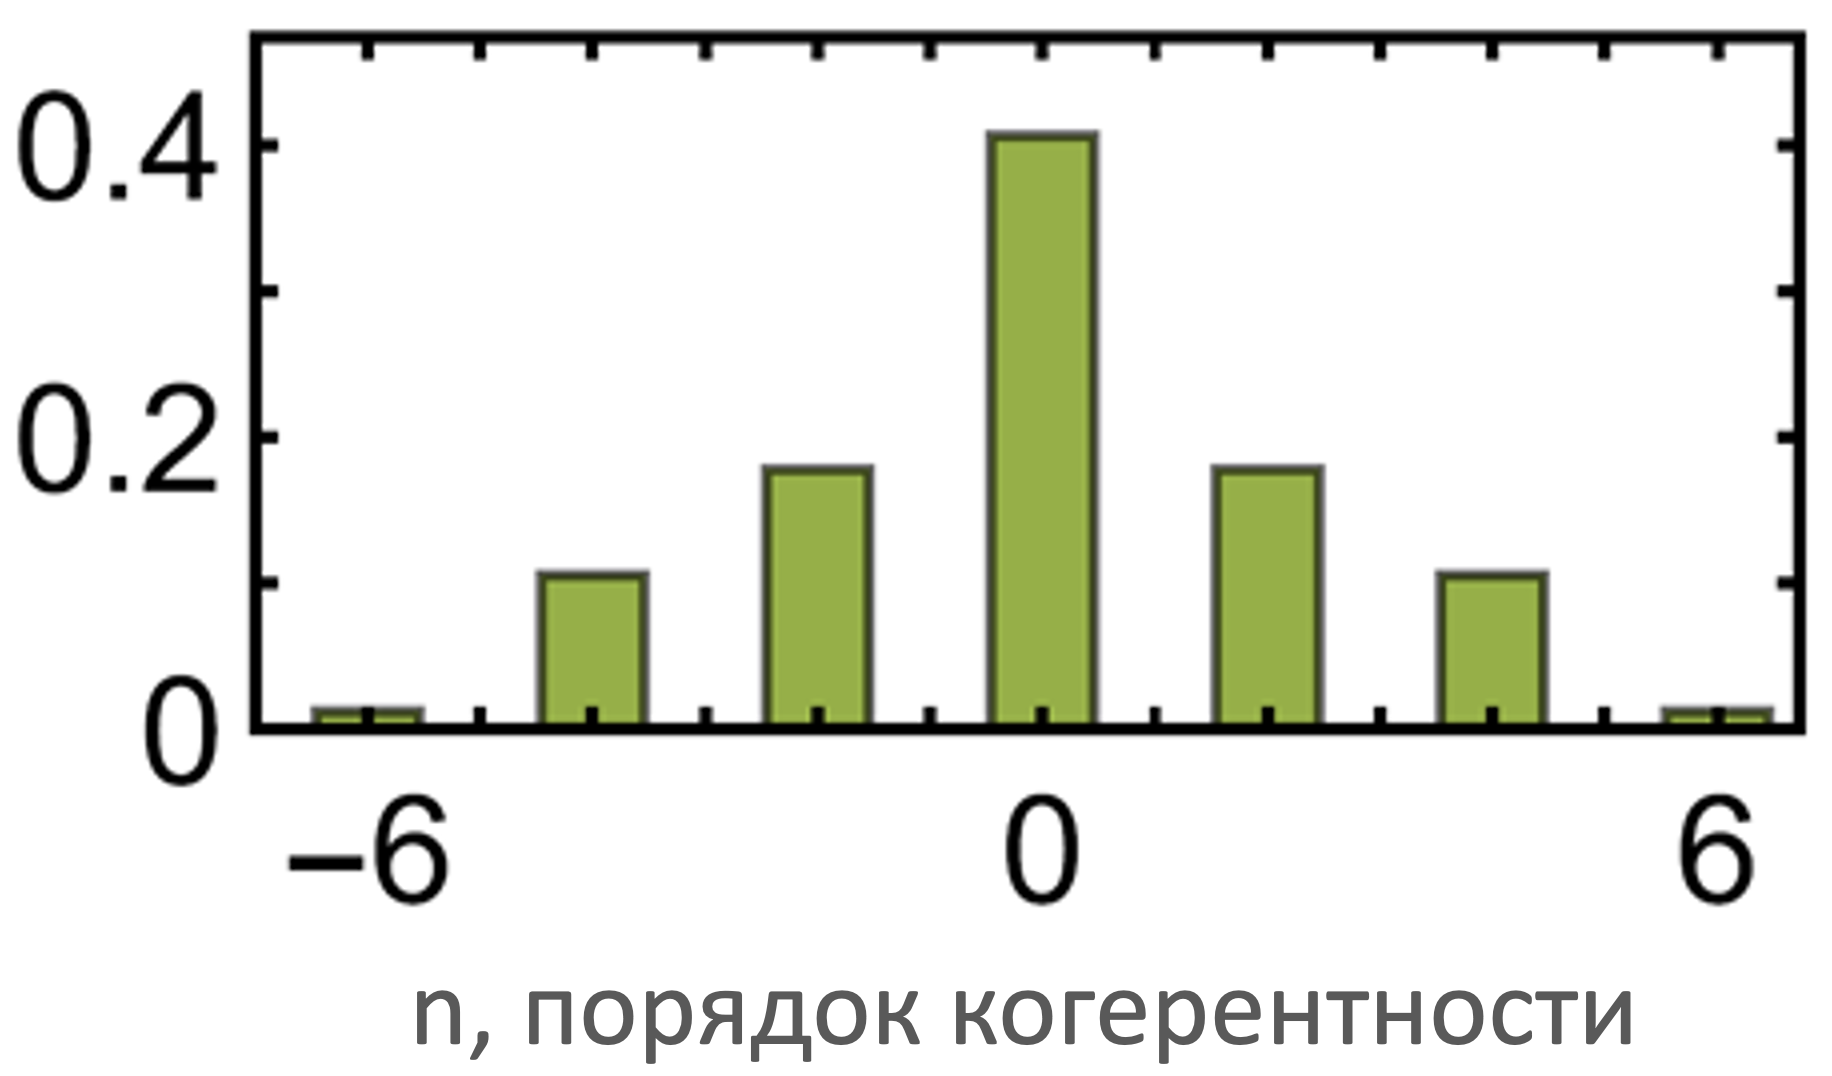
\includegraphics[width=\textwidth]{mq-coherence-intensities-hist.png}
%     \caption{Распределение интенсивности МК когерентностей ЯМР.}
%     \label{fig:distribution}
% \end{figure}
%

В разделе~\ref{sec:quantum-fisher-information} было показано,
что величина квантовой информации Фишера определяет нижнюю границу числа запутанных частиц в системе.
Дальнейшее исследование многочастичной запутанности требует
разработки экспериментальных методов измерения квантовой информации Фишера.
В этом разделе будет показано,
что удвоенный второй момент распределения МК когерентностей ЯМР,
которые возникают на подготовительном периоде МК эксперимента ЯМР
(см. раздел~\ref{sec:mq-nrm-experiment}),
определяет нижнюю границу квантовой информации Фишера~\cite{Garttner2018}.

Пусть система в начальный момент времени находится в термодинамическом равновесии,
тогда матрица плотности системы имеет вид
%
\begin{equation}
  \label{eq:rho_eq}
  \rho(0)
  = \rho_{\mathrm{eq}}
  = \dfrac{
    e^{\frac{\hbar\omega_{0}}{kT} I_z}
  }{
    \tr{e^{\frac{\hbar\omega_{0}}{kT} I_z}}
  }
  \approx \dfrac{1}{2^N} (1 + bI_z)
  \sim I_z.
\end{equation}
%
Эволюционная матрица плотности на подготовительном периоде МК эксперимента ЯМР,
где динамика определяется стационарным МК гамильтонианом $H_\mathrm{MQ}$,
может быть выражена как
%
\begin{equation}\label{eq:rho_eval_ht}
  \rho_\mathrm{HT} (\tau)
   =  e^{-iH_\mathrm{MQ}\tau} I_z e^{iH_\mathrm{MQ}\tau}.
\end{equation}
%
С учетом Ур.~(\ref{eq:rho_eval_ht}) выражение~(\ref{eq:signal-after-mixing})
финального сигнала МК эксперимента ЯМР $G_\mathrm{HT}(\tau,\phi)$ можно переписать в виде
%
\begin{multline}\label{eq:signal-after-mixing-ht}
  G_\mathrm{HT}(\tau,\phi)
  = \tr{
  	e^{iH_{MQ}\tau} e^{i\phi I_z} e^{-iH_{MQ}\tau} I_z
  	e^{iH_{MQ}\tau} e^{-i\phi I_z} e^{-iH_{MQ}\tau} I_z
  }
  \\
  = \tr{
    e^{i\phi I_z} \rho_\mathrm{HT}(\tau)
    e^{-i\phi I_z}\rho_\mathrm{HT}(\tau)
  }.
\end{multline}
%
Из выражения~(\ref{eq:signal-after-mixing-ht}) следует,
что $G_\mathrm{HT}(\tau, \phi)$ является неупорядоченным по времени коррелятором ``out-of-time ordered correlator'' (OTOC)~\cite{Garttner2018, Doronin2019}.
Важно отметить, что данное свойство является ключевым в доказательстве связи
второго момента МК спектра ЯМР и квантовой информации Фишера.
Все дальнейшие рассуждения будут опираться на него.

Второй момент (дисперсия) $M_2(\tau)$ распределения интенсивностей МК когерентностей ЯМР может быть рассчитан из уравнения ~(\ref{eq:signal-after-mixing-ht})
\begin{equation}\label{eq:m2-derivative}
  M_2(\tau)
  = -\frac{1}{G_\mathrm{HT}(\tau, 0)}
    \frac{d^2 G_\mathrm{HT}(\tau, \phi)}{d\phi^2}\bigg|_{\phi=0}.
\end{equation}
%
Для этого разложим выражение~(\ref{eq:signal-after-mixing-ht})
для сигнала~$G_\mathrm{HT}(\tau,\phi)$ в ряд по инкременту фазы импульсов
%
% \begin{equation}\label{eq:17}
% \begin{split}
\begin{multline}
  G_\mathrm{HT}(\tau,\phi)
  = \tr{
    \rho_\mathrm{HT}(\tau) e^{i \phi I_\mathrm{z} }
    \rho_\mathrm{HT}(\tau) e^{-i\phi I_\mathrm{z} }
  } \\
  =  \tr{
    (1 - iI_z\phi - \frac{1}{2} I_z^2 \phi^2)
    \rho_\mathrm{HT}(\tau)
    (1 + iI_z\phi - \frac{1}{2} I_z^2 \phi^2)
    \rho_\mathrm{HT}(\tau)
  } \\
  = \tr{
    \rho_\mathrm{HT}^2
    - it [I_z,\rho_\mathrm{HT}(\tau)]
    + \phi^2 I_z \rho_\mathrm{HT}(\tau) I_z \rho_\mathrm{HT}(\tau)
    - \frac{\phi^2}{2} I_z^2 \rho_\mathrm{HT}^2(\tau)
    - \frac{\phi^2}{2} \rho_\mathrm{HT}(\tau) I_z^2 \rho_\mathrm{HT}(\tau)
  } \\
  = \tr{ \rho_\mathrm{HT}^2(\tau) }
  - \phi^2 \tr{
    \rho_\mathrm{HT}^2(\tau) I^2_\mathrm{z}
    - (\rho_\mathrm{HT}(\tau) I_\mathrm{z})^2
  }
  + O(\phi^3).
\end{multline}
% \end{split}
% \end{equation}
%
Отсюда второй момент распределения МК когерентностей ЯМР
%
\begin{equation}\label{eq:m2-trace}
  M_{2,\mathrm{HT}}(\tau) = 2 \tr{
    \rho_\mathrm{HT}(\tau)^2 I_z^2
    - \rho_\mathrm{HT}(\tau) I_z \rho_\mathrm{HT}(\tau) I_z
  },
\end{equation}
%
так как в МК эксперименте ЯМР сумма всех интенсивностей нормируется на 1
и
\begin{equation}\label{eq:mq-coherences-sum}
  G_\mathrm{HT}(\tau, 0)
  = \tr{\rho_\mathrm{HT}(\tau)^2}
  = \tr{\sum\limits_{n,m} \rho_n \rho_m}
  = \tr{\sum\limits_{n} \rho_n \rho_{-n}}
  = \sum_n J_n (\tau) \equiv 1,
\end{equation}
где $\rho_n$ --- это вклад МК когерентности $n$-ого порядка в матрицу плотности $\rho_\mathrm{HT}(\tau)$,
а $J_n$ --- интенсивность МК когерентности $n$-ого порядка.
%
Выражение~(\ref{eq:m2-trace}) для второго момента $M_{2,\mathrm{HT}}(\tau)$
может быть выражено через собственные значения $\lambda_i$ матрицы плотности $\rho_\mathrm{HT}(\tau)$:
%
\begin{equation}\label{eq:m2-via-lambdas}
\begin{split}
  M_{2,\mathrm{HT}}(\tau)
  &= 2 \sum_{j,k}\p{\lambda^2_j (I_z)_{jk} (I_z)_{kj} - \lambda_j (I_z)_{jk} \lambda_k (I_z)_{kj}}
  \\
  &= 2 \sum_{j,k} (\lambda^2_j - \lambda_j \lambda_k) (I_z)_{jk} (I_z)_{kj}
  \\
  &= \sum_{j,k} (\lambda^2_j - \lambda_j \lambda_k) (I_z)_{jk} (I_z)_{kj}
    + \sum_{j,k} (\lambda^2_j - \lambda_j \lambda_k) (I_z)_{kj} (I_z)_{jk}
  \\
  &= \sum_{j,k}
    (\lambda^2_j - 2\lambda_j \lambda_k + \lambda^2_k)
    (I_z)_{kj} (I_z)_{jk}
  \\
  &= \sum_{j,k}
    (\lambda_j - \lambda_k)^2
    \left| \bra{j} I_z \ket{k} \right|^2.
\end{split}
\end{equation}
%
По определению~\ref{def:quantum-fisher-information} квантовая информация Фишера дается выражением
\begin{equation}
    F_Q(\rho_\mathrm{HT}(\tau), I_z) = 2\sum_{j,k} \frac{(\lambda_j - \lambda_k)^2}{\lambda_j + \lambda_k}
    \left| \bra{j} I_z \ket{k} \right|^2.
\end{equation}
Поскольку $\tr{\rho_\mathrm{HT}} = 1$, $\lambda_j + \lambda_k \leq 1$ и
%
\begin{equation}\label{eq:qfi-low-bound}
  F_Q(\rho_\mathrm{HT}(\tau), I_z) \geq 2\sum_{j,k} (\lambda_j - \lambda_k)^2 \left| \bra{j} I_z \ket{k} \right|^2.
\end{equation}
%
Из выражений~(\ref{eq:qfi-low-bound})~и~(\ref{eq:m2-via-lambdas}) следует, что
\begin{equation}
  F_Q(\rho_\mathrm{HT}(\tau), I_z) \geq 2 M_{2,\mathrm{HT}}(\tau).
\end{equation}
%
Таким образом, нижняя граница информации Фишера равна удвоенному второму моменту.

Данный результат получен в случае высоких зеемановских температур,
когда начальное состояние системы $I_z$.
В свою очередь квантовые корреляции преимущественно возникают при температурах близких к нулю.
В следующей главе~\ref{chapter:quantum-fisher-information-measurement}
будет обсуждено такое обобщение МК эксперимента ЯМР,
которое позволяет измерять информацию Фишера при произвольной температуре.
